\documentclass[a4paper]{report}

\newlength{\addtextwidth}
\newlength{\addtextheight}
\setlength{\addtextwidth}{16.0cm}
\setlength{\addtextheight}{22.3cm}
\addtolength{\addtextwidth}{-\textwidth}
\addtolength{\addtextheight}{-\textheight}

\addtolength{\textheight}{\addtextheight}
\addtolength{\textwidth}{\addtextwidth}
\addtolength{\oddsidemargin}{-0.5\addtextwidth}
\addtolength{\evensidemargin}{-0.5\addtextwidth}
\addtolength{\topmargin}{-0.15\addtextheight}


\newcommand{\book}[3]{\noindent{\sf #1} {\it #2} #3

 \medskip

}
\newcommand{\article}[4]{\noindent{\it #1} {\bf #2} {\sf #3} #4

\medskip

}
\newcommand{\PH}{P\!H}
\newcommand{\Ref}{\bigskip \noindent {\large\bf References} \medskip }
\newcommand{\Proof}{{\sc Proof}}
\newcommand{\NP}{N\!P}
\newcommand{\p}{\hspace{-0.90ex}.\hspace{0.90ex}}
\newcommand{\qed}{\hfill $\Box$ \hspace{1.1ex}}
\newcommand{\CC}[1]{}

%\newcommand{\N}{\mbox{\boldmath\(N\)}}
%\newcommand{\Z}{\mbox{\boldmath\(Z\)}}
%\newcommand{\Q}{\mbox{\boldmath\(Q\)}}
%\newcommand{\R}{\mbox{\boldmath\(R\)}}
%\newcommand{\C}{\mbox{\boldmath\(C\)}}



\newtheorem{defii}{Definition}
\newtheorem{teo}{Theorem}
\newtheorem{lema}{Lemma}
\newtheorem{obs}{Observation}
\newtheorem{coro}{Corollary}
\newtheorem{conj}{Conjecture}
\newtheorem{claim}{Claim}
%\documentclass[psfig,12pt,fullpage,twoside,fancyheadings]{report}
%\documentstyle[12pt,fullpage]{article}

%\pagestyle{fancy}
\renewcommand{\sectionmark}[1]{\markboth{#1}{#1}} % remember chapter title
\renewcommand{\subsectionmark}[1]{\markright{\thesubsection\ #1}}
                                                % section number and title
%\lhead[\fancyplain{}{\bf\thepage}]{\fancyplain{}{\bf\rightmark}}
%\rhead[\fancyplain{}{\bf\leftmark}]{\fancyplain{}{\bf\thepage}}
%\cfoot{}

%\addtolength{\textheight}{-3.6in}
%\addtolength{\voffset}{-0.5in}

%%% Local Variables:
%%% mode: latex
%%% TeX-master: "math-faq"
%%% End:

\usepackage[utf8]{inputenc}
\usepackage{graphicx}
\usepackage{amssymb}
\usepackage{xspace}
\usepackage[osf]{mathpazo}
\usepackage[backref]{hyperref}
\usepackage[chapter]{algorithm}
\usepackage{algorithmic}
\usepackage{chapterbib}

\title{Frequently Asked Questions in Mathematics}
\author{The \href{news://sci.math}{\texttt{sci.math}} FAQ Team\\
  \bigskip
  {\small Editors:}\\
  \bigskip
  {\small Alex L\'{o}pez-Ortiz, \url{alopezo@unb.ca}}\\
  {\small Rog\'{e}rio Theodoro de Brito, \url{rbrito@ime.usp.br}}
}

\begin{document}
\maketitle
\tableofcontents

%* 1 Introduction
%* 2 Fundamentals
%    FAQ section What are numbers?,
%    The Axiom of Choice,
%    The Continuum Hypothesis
%* 3 Number Theory
%    FAQ section Fermat's Last Theorem,
%    Special Numbers and Functions but not Indiana bill,
%    Prime Numbers
%* 4 Human Interest
%    FAQ section Indiana bill sete the value of Pi to 3,
%    Fields Medal,
%    Mathematical Oddities.
%* 5 Mathematical Trivia
%    FAQ section Names of large numbers,
%    Projective Plane of Order 10,
%    Theory of quaternionic analytic functions,
%    Which are the 23 Hilbert Problems?
%* 6 Problems & Games
%    FAQ section Names of large numbers,
%    Famous Problems in Mathematics, including Hilbert's.
%    Mathematical Games
%* 7 Miscellaneous
%    FAQ section Formulas of General Interest,
%    Symbolic Computation,
%    General Bibliography and Textbooks
%* 8 Contributors
%    FAQ section Sci.Math FAQ Team,
%    Copyright Notice.

\chapter{Introduction}
  \section{Why a list of Frequently Asked Questions?}

\emph{The Net}, as users call the Internet, and specially
\emph{newsgroups}, (i.e., Usenet) created a demand of knowledge without
parallel since the invention of the printing press.  Surprisingly, the
type of knowledge demanded from and by the Usenet community had, in most
cases, little in common---both in structure and content---with that of
printed in current publications. This defined Usenet as more of an
alternative to books rather than a replacement thereof.\footnote{It
  could be argued that books fulfill their mandate and purpose to
  everybody's satisfaction.  Thus, even though the Net could, in
  principle, replace the need for books, people choose not to do
  so. Instead it's domain is defined, by its very nature to be disjoint
  from books.}

In the Net, questions posed are, more often than not, at the level of an
amateur practitioner---even in cases where the question was posed by a
professional in the field. Similarly, the quality of the answers varies
greatly, ranging from the incorrect or disrespectful, to summaries of
the state of the art in the topic in question.

Other characteristics of communication on the Net are simply inherited
from restrictions of the medium. The unit of knowledge is a screenful
worth of text (a scrit, from screen and bit). Articles exceeding that
limit are usually disregarded.

The lack of memory of the medium generates a repetition of topics, much
to the chagrin of old time citizens of the Net.  Frequently asked
questions (FAQ) lists palliate some of these deficiencies by providing a
record of relevant information while at the same time never being
outdated.\footnote{Or, at least, the editors would like to think so!}

Thus, typically a list of frequently asked questions is ``posted'' at
least once a month, and updated at least as frequently. And, in what
must be a first for an information based product, FAQ lists ``expire''
on a given date, very much like any other perishable item.


\section{Frequently Asked Questions in Mathematics?}

If I had to describe the contents of the FAQ in Mathematics in a single
sentence, I would call it \emph{mathematical gossip} or perhaps
\emph{non-trivial mathematical trivia}.

The FAQ list is a compilation of knowledge of interest to most
professional and amateur mathematicians, ranging from advanced topics
such as Wiles' proof to Fermat's Last Theorem to the list of Fields
Medal winners.

%%% Local Variables: 
%%% mode: latex
%%% TeX-master: "math-faq"
%%% End: 

\chapter{Fundamentals}
  \newcommand{\N}{\ensuremath{\mathbb N}\xspace}
\newcommand{\Z}{\ensuremath{\mathbb Z}\xspace}
\newcommand{\Q}{\ensuremath{\mathbb Q}\xspace}
\newcommand{\R}{\ensuremath{\mathbb R}\xspace}
\newcommand{\C}{\ensuremath{\mathbb C}\xspace}

%%% Local Variables: 
%%% mode: latex
%%% TeX-master: "math-faq"
%%% End: 

  \section{Algebraic structures}

We will attempt to give a brief explanation of the following concepts:
\begin{itemize}
  \item \N is a monoid
  \item \Z is an integral domain
  \item \Q is a field
  \item in the field \R the order is complete
  \item the field \C is algebraically complete
\end{itemize}

If you have been asked by a child to give them arithmetic problems, so
they could show off their newly learned skills in addition and
subtraction I'm sure that after a few problems such as: $2 + 3$, $9 -
5$, $10 + 2$ and $6 - 4$, you tried tossing them something a little more
difficult: $4 - 7$ only to be told ``{\it That's not allowed.}''

What you may not have realized is that you and the child did not just
have different objects in mind (negative numbers) but entirely different
{\it algebraic systems}. In other words a set of objects (they could be
natural numbers, integers or reals) and a set of operations, or rules
regarding how the numbers can be combined.

We will take a very informal tour of some algebraic systems, but before
we define some of the terms, let us build a structure which will have
some necessary properties for examples and counterexamples that will
help us clarify some of the definitions.

We know that any number that is divided by six will either leave a
remainder, or will be divided exactly (which is after all the remainder
0). Let us write any number by the remainder $n$ it leaves after
division by six, denoting it as $[ n ]$. This means that, $7, 55$ and
$1$ will all be written $[1]$, which we call the {\it class} to which
they all belong: i.e. $7 \in [1]$, $55 \in [1]$, or, a bit more
technically, they are all equivalent to 1 modulo 6.  The complete set of
class will contain six elements, and this is called partitioning numbers
into equivalent classes because it separates (or partitions) all of our
numbers into these classes, and any one number in a class is equivalent
to any other in the same class.

One interesting thing we can do with these classes is to try to add or
to multiply them. What can $[1] + [3]$ mean? We can, rather naively try
out what they mean in ``normal'' arithmetic: $[1] + [3] = [1+3] = [4]$.
So far so good, let us try a second example $25 \in [1]$ and $45 \in
[3]$, their sum is $70$ which certainly belongs to $[4]$. Here we see
what we meant above by equivalence, 25 is equivalent to 1 as far as this
addition is concerned. Of course this is just one example, but
fortunately it can be proven that the sum of two classes is always the
class of the sums.

Now this is the kind of thing we all do when we add hours for example, 7
(o' clock) plus 6 hours is 1 (o' clock), and all we are really doing is
adding hours (modulo 12).

The neat part comes with multiplication, as we will see later on. But
for now just remember, it can be proven that something like $[4] \times
[5] = [2]$ will work: the product of two classes is the class of the
product.

Now for some of the necessary terminology.

\subsection{Monoids and Groups}

We need to define a {\em group}.

Let us take a set of objects and a rule (called a binary operation)
which allows us to combine any two elements of this set. Addition is an
example from math, or ANDing in some computer language.

The set must be closed under the operation. That means that when two
elements are combined the result must also be in the set. For example
the set containing even numbers will always give us an even number when
two elements are added together. But if we restrict ourselves to odd
numbers, their sum is not an odd number and so we know right off the bat
that the set of odd numbers and addition cannot constitute a group. Some
books will consider closure in the definition of binary operation, and
others add it as one of the requirements for a group along with the ones
that follow below.

The set and the operation is called a group if the binary operation
satisfies the following criteria:
\begin{itemize}
  \item the operation is associative, which means it doesn't matter how
  you group the elements you are operating on, for example in our set of
  remainders: $[1] + ([3] + [4]) = ([1] + [3]) + [4]$
  \item there is an identity element, meaning: one of the elements
  combined with the others in the set doesn't change them in the
  least. For example the zero in addition, or the one in multiplication.
  \item every element has an inverse with respect to that operation. If
  you combine an element and its inverse you get the identity (of that
  operation) back.
\end{itemize}

(Be careful with this last one, $-3$ is the inverse of $3$ in addition,
since they give us 0 when added, but $1/3$ is the inverse of 3 with
respect to multiplication, since $3 \times 1/3 = 1$ the identity under
multiplication.)

So we can see that the set of natural numbers \N (with the operation of
addition) is not even a group, since there is no inverse for 5, for
example.  (In other words there is no natural number which added to 5
will give us zero.) And so the third rule for our operation is violated.
But it still has \emph{some} structure, even if it is not as rich as the
ones we'll see later on.

Sets with an associative operation (the first condition above) are
called semigroups, and if they also have an identity element (the second
condition) then they are called monoids.

Our set of natural numbers under addition is then an example of a
monoid, a structure that is not quite a group because it is missing the
requirement that every element have an inverse under the operation
(Which is why in elementary school $4 - 7$ is not allowed.)

What about the set of integers, is it a group?

By itself this question is nonsensical. Why? Well, we have not mentioned
under what operation. OK, let us say: the set of integers with addition.

Now, addition is associative, the zero does not change any number when
added to it, and for every number $n$ we can add $-n$ and get zero. So
it's a group all right.

In fact it is a special kind of group. When we can perform the operation
on the two elements in any order (e.g $a + b = b + a$) then the group is
called commutative, or {\em Abelian} in honor of Abel. Not every
operation is commutative, for example three minus two is certainly {\em
  not} the same as two minus three. Our set of integers under addition
is then an Abelian group.


\subsection{Rings}

If we take an Abelian group (remember: a set with a binary operation)
and we define a second operation on it we get a bit more of a structure
than we had with just a group.

If the second operation is associative, and it is distributive over the
first then we have a ring. Note that the second operation may not have
an identity element, nor do we need to find an inverse for every element
with respect to this second operation. As for what distributive means,
intuitively it is what we do in math when perform the following change:
$a \times (b + c) = (a \times b) + (a \times c)$.

If the second operation is also commutative then we have what is called
a commutative ring. The set of integers (with addition and
multiplication) is a commutative ring (with even an identity---called
unit element---for multiplication).

Now let us go back to our set of remainders. What happens if we multiply
$[5] \times [1]$? We see that we get $[5]$, in fact we can see a number
of things according to our definitions above, $[5]$ is its own inverse,
and $[1]$ is the multiplicative element. We can also show easily enough
(by creating a complete multiplication table) that it is
commutative. But notice that if we take $[3]$ and $[2]$, neither of
which are equal to the class that the zero belongs to $[0]$, and we
multiply them, we get $[3] \times [2] = [0]$.  This bring us to the next
definition. In a commutative ring, let us take an element which is not
equal to zero and call it $a$. If we can find a non-zero element, say
$b$ that combined with $a$ equals zero ($a \times b = 0$) then $a$ is
called a {\it zero divisor}.

A commutative ring is called an integral domain if it has no zero
divisors.  Well the set \Z{} with addition and multiplication fullfills
all the necessary requirements, and so it is an integral domain. Notice
that our set of remainders is not an integral domain, but we can build a
similar set with remainders of division by five, for example, and
voil\`a, we have an integral domain.

Let us take, for example, the set \Q{} of rational numbers with addition
and multiplication - I'll leave out the proof that it is a ring, but I
think you should be able to verify it easily enough with the above
definitions. But to give you a head start, notice the addition of
rationals follow all the requirements for an abelian group. If we remove
the zero we will have another abelian group, and that implies that we
have something more than a ring, in fact, as we will see in the next
section.

\subsection{Fields}

Now we can make one step further. If the elements of a ring, excluding
the zero, form an abelian group (with the second operation) then it is a
field.  For example, write the multiplication table of the remainders of
division by 5, and you will see that it satisfies all the requirements
for a group: (You will probably have noticed that the group does not
contain the number five itself since $[5] = [0]$.)
\[
\begin{tabular}{  c  |  c  c  c  c  }
    & 1 & 2 & 3 & 4  \\
    \hline
  1 & 1 & 2 & 3 & 4 \\
  2 & 2 & 4 & 1 & 3 \\
  3 & 3 & 1 & 4 & 2 \\
  4 & 4 & 3 & 2 & 1
\end{tabular}
\]

(Why isn't the set of divisors of six---excluding the zero and under
multiplication---a group?  That's easy enough, since we have excluded
the zero we do not have the result of $[2] \times [3]$ in our set, so it
isn't closed.)

\subsection{Ordering}

Given a ring, we can say that it is ordered when you have a special
subset of that ring behaves in a very special way. If any two elements
of that special subset are added or multiplied their sum and their
product are again in the special subset. Take the negative numbers in
\R{}, can they be that special subset? Well the sum seems to be
allright, it is also a negative number. But things don't work with the
product: it is positive. What about the positive numbers? Yep, and in
fact we call that special subset, the set of positive elements. Now, we
gave the definition for an ordered ring, we can also define an ordered
field the same way.

But what does a complete ordered field mean? Well the definition looks
rather nasty: it is complete if every non-empty subset which posesses an
upper bound has a least upper bound.

Let's translate some of that, trying to lose as little information on
the way. A bound is something that guarantees that all of the elements
of your set are on one side of it (reasonably enough). For example,
certainly all negative reals are less than 100, so 100 is a bound (it is
in fact an upper bound 'cause all negatives are ``below'' it). But there
are lots of other bounds, 1, 5, 26 will all do nicely. The question now
is, of all of these (upper bounds) which is the smallest, that is which
one is ``the border'' so to speak? Does it always exists?

Let's take the rationals, and look at the following numbers:
\[1.4, \; 1.41, \; 1.414, \; 1.4142, \; 1.41421, \ldots \]

Now each of these is a rational number (it can be written as a
fraction), and they are getting closer and closer to a number we've
probably seen before (just take out your calculator and find the square
root of two).  So we can write the shorthand for this series as
$\sqrt{2}$.  Certainly we can find an upper bound for this series, $3$
will do nicely, but so can $1.5$, or $1.42$. But what is the
smallest. Well there isn't any. Not among the rational at least, because
no matter what fraction you give I can give you one closer to the square
root of two. What about the square root of two itself? Well it's not a
rational number (I'll skip the proof, but it is really rather easy) so
you can't use it.  If you want another series which is really neat look
at the section on ``Euler's formula'' in the FAQ.

And that is where the reals come in. Any set or reals that is bounded
you can certainly find the smallest of these bounds. (By the way this
``least upper bound'' is abbreviated ``l.u.b.'', or ``sup'' for {\it
  supremum}.) We can also turn things around and talk of lower bounds,
and of the largest of these etc. but most of that will be just a mirror
image of what we have dealt with so far.

So that should be it. And for years that did seem to be it, we seemed to
have all the numbers we'd ever care to have.

There was just one small stick in the works, but most people just sort
of pretended not to notice, and that was that not all polynomials had
solutions. One simple polynomial of this kind is $x^2 + 1 = 0$.  It's so
simple, yet there's no self respecting number that would solve this
polynomial. There were these funny answers which seemed like they should
be solutions but no one could make any sense out of them, so they were
considered imaginary solutions.  Which was really too bad because they
were given the name of imaginary numbers and now that the name stuck we
realize that they are numbers just as good as any of the ones we have
been using for centuries. And in fact that takes us to the last great
pinnacle in this short excursion. The field of complex numbers.

We can define an algebraically closed field as a field where every
nonconstant polynomial (i.e. one with an $x$ in it from high school
days) has a zero in the field. Whew! This in short means that as long as
the polynomial is not a constant number (which is no fun anyways) but
something which looks like it wants a solution, like $5 x^3 - 2 x^2 + 6
= 0$ it will always have one, if you are working with complex numbers
and not just reals.


There is another definition which is probably just as good, but may or
may not be easier: A field is algebraically closed if every polynomial
splits into linear factors.  Linear factors are briefly factors not
containing $x$ to any power of two or higher, in other words in the
form: $ax + b$. For example $x^2 + x -6$ can be factored as $(x + 3)(x -
2)$, but if we are in the field of reals we cannot factor $x^2 + 1$, but
we can in the field of complex numbers: $x^2 + 1 = (x - i)(x + i)$,
where, you may recall, $i^2 = -1$.
%%% Local Variables:
%%% mode: latex
%%% TeX-master: "math-faq"
%%% End:

  \section{What are numbers?}

\subsection{Introduction}

Informally:
\begin{itemize}
  \item $\N = \{0,1,\ldots\}$ or $\N = \{1,2,\ldots\}$ \\
  Wether $0$ is in $\N$ depends on where you live and what is your field
  of interest. At the informal level it is a religious topic.
  \item $\Z = \{\ldots,-1,0,1,\ldots\}$
  \item $\Q = \{p/q | p, q \in \Z \mbox{ and } q \neq 0\}$
  \item $\R = \{d_0.d_1d_2\ldots | d_0 \in \Z \mbox{ and } 0 \leq d_i
  \leq 9 \mbox{ for } i>0\}$
  \item $\C = \{a+b \cdot i | a, b \in \R \mbox{ and } i^2 = -1\}$
\end{itemize}

\subsection{Construction of the Number System}

% Credit: mmcadams@cco.caltech.edu (Matt McAdams) 951209
%         main stream --> mainstream

Formally (following the mainstream in math) the numbers are constructed
from scratch out of the axioms of Zermelo Fraenkel set theory (a.k.a.\
ZF set theory) [Enderton77, Henle86, Hrbacek84]. The only things that
can be derived from the axioms are sets with the empty set at the bottom
of the hierarchy.  This will mean that any number is a set (it is the
only thing you can derive from the axioms). It doesn't mean that you
always have to use set notation when you use numbers: just introduce the
numerals as an abbreviation of the formal counterparts.

% Credit: aaron@mmml.demon.co.uk (Aaron Turner) 950330
%         He suggested numerals as an alternative for ``informal'' numbers.

% Credit: mcknighl@ix.netcom.com (Lawrence McKnight) 941104
%         He asked to add rationales to the constructions.

The construction starts with $\N$ and algebraically speaking, $\N$ with
its operations and order is quite a weak structure. In the following
constructions the structures will be strengthen one step at the time:
$\Z$ will be an integral domain, $\Q$ will be a field, for the field
$\R$ the order will be made complete, and field $\C$ will be made
algebraically complete.
% Credit: aaron@mmml.demon.co.uk (Aaron Turner) 950330
%         He asked for a brief explanation. This is as for as I'll go:
%
% [Is there a volunteer in the crowd who likes to write a section that
% explains these structures and concepts?]
%
% Yep, there is: andrea.depaoli@mail.esrin.esa.it (Andy de Paoli) 951102
% So these lines are removed and Andy's part is added by Alex to the FAQ.

Before we start, first some notational stuff:
\begin{itemize}
  \item a pair $(a,b) = \{\{a\},\{a,b\}\}$,
  \item an equivalence class $[a] = \{b | a \equiv b\}$,
  \item the successor of $a$ is $s(a) = a \cup \{a\}$.
\end{itemize}
% Credit: aaron@mmml.demon.co.uk (Aaron Turner) 950330
%         He liked to put a little more stress on the fact that other
%         definitions are possible (although this is the de facto one.

Although the previous notations and the constructions that follow are
the de facto standard ones, there are different definitions possible.

\subsection{Construction of \sl $N$}

\begin{itemize}
  \item $\{\} \in \N$
  \item if $a \in \N$ then $s(a) \in \N$
  \item $\N$ is the smallest possible set such that the preceding rules
  hold.
\end{itemize}
Informally $n=\{0,\ldots,n-1\}$ (thus $0=\{\}$, $1=\{0\}$, $2=\{0,1\}$,
$3=\{0,1,2\}$). We will refer to the elements of $\N$ by giving them a
subscript $_n$. The relation $<_n$ on $\N$ is defined as: $a_n <_n b_n$
iff $a_n \in b_n$. We can define $+_n$ as follows:
\begin{itemize}
  \item $a_n +_n 0_n = a_n$
  \item $a_n +_n s(b_n) = s(a_n +_n b_n)$
\end{itemize}
Define $*_n$ as:
\begin{itemize}
  \item $a_n *_n 0_n = 0_n$
  \item $a_n *_n s(b_n) = (a_n *_n b_n) +_n a_n$
\end{itemize}

\subsection{Construction of \sl Z}

We define an equivalence relation on $\N \times \N$: $(a_n,b_n) \equiv_z
(c_n,d_n)$ iff $a_n +_n d_n = c_n +_n b_n$. Note that $\equiv_z$
``simulates'' a subtraction in $\N$. $\Z = \{[(a_n,b_n)]_z | a_n, b_n
\in \N\}$. We will refer to the elements of $\Z$ by giving them a
subscript $_z$.  The elements of $\N$ can be embedded as follows:
$embed_n: \N \rightarrow \Z$ such that $embed_n(a_n) =
[(a_n,0_n)]_z$. Furthermore we can define:
\begin{itemize}
  \item $[(a_n,b_n)]_z <_z [(c_n,d_n)]_z$ iff $a_n +_n d_n <_n c_n +_n b_n$
  \item $[(a_n,b_n)]_z +_z [(c_n,d_n)]_z = [(a_n +_n c_n, b_n +_n d_n)]_z$
  \item $[(a_n,b_n)]_z *_z [(c_n,d_n)]_z =$ \\
        $[\left((a_n *_n c_n) +_n (b_n *_n d_n), (a_n *_n d_n) +_n (c_n *_n
          b_n)\right)]_z$
\end{itemize}

\subsection{Construction of \sl Q}

We define an equivalence relation on $\Z \times (\Z \backslash
\{0_z\})$: $(a_z,b_z) \equiv_q (c_z,d_z)$ iff $a_z *_z d_z = c_z *_z
b_z$. Note that $\equiv_q$ ``simulates'' a division in $\Z$. $\Q =
\{[(a_z,b_z)]_q | a_z \in \Z \mbox{ and } b_z \in \Z \backslash
\{0_z\}\}$. We will refer to the elements of $\Q$ by giving them a
subscript $_q$. The elements of $\Z$ can be embedded as follows:
$embed_z: \Z \rightarrow \Q$ such that $embed_z(a_z) =
[(a_z,1_z)]_q$. Furthermore we can define:
\begin{itemize}
  \item $[(a_z,b_z)]_q <_q [(c_z,d_z)]_q$ iff $a_z *_z d_z <_z c_z *_z b_z$
  when $0_z <_z b_z \mbox{ and } 0_z <_z d_z$
  \item $[(a_z,b_z)]_q +_q [(c_z,d_z)]_q = [\left((a_z *_z d_z) +_z (c_z *_z
    b_z), b_z *_z d_z\right)]_q$
  \item $[(a_z,b_z)]_q *_q [(c_z,d_z)]_q = [(a_z *_z c_z, b_z *_z d_z)]_q$
\end{itemize}

\subsection{Construction of \sl R}

The construction of $\R$ is different (and more awkward to understand)
because we must ensure that the cardinality of $\R$ is greater than that
of $\Q$.

Set $c$ is a {\em Dedekind cut} iff
\begin{itemize}
  \item $\{\} \subset c \subset \Q$ (strict inclusions!)
  \item $c$ is {\em closed downward}: \\
  if $a_q \in c$ \mbox{ and } $b_q <_q a_q$ then $b_q \in c$
  \item $c$ has no {\em largest element}: \\
      there isn't an element $a_q \in c$ such that $b_q <_q a_q$ for all $b_q
      \neq a_q \in c$
\end{itemize}

You can think of a cut as taking a pair of scissors and cutting $\Q$ in
two parts such that one part contains all the small numbers and the
other part contains all large numbers. If the part with the small
numbers was cut in such a way that it doesn't have a largest element, it
is called a Dedekind cut.  $\R = \{c | c \mbox{ is a Dedekind
  cut}\}$. We will refer to the elements of $\R$ by giving them a
subscript $_r$. The elements of $\Q$ can be embedded as follows:
$embed_q: \Q \rightarrow \R$ such that $embed_q(a_q) = \{b_q | b_q <_q
a_q\}$. Furthermore we can define:

\begin{itemize}
  \item $a_r <_r b_r$ iff $a_r \subset b_r$ (strict inclusion!)
  \item $a_r +_r b_r = \{c_q +_q d_q | c_q \in a_r \mbox{ and } d_q \in b_r\}$
  \item $-_r a_r = \\
  \{b_q |$ there exists an $c_q \in \Q$ such that $b_q <_q c_q \mbox{ and
  } (-1)_q *_q c_q \not\in a_r\}$
  \item $|a_r|_r = a_r \cup -_r a_r$
  \item $*_r$ is defined as:
  \begin{itemize}
    \item if not $a_r <_r 0_r$ and not $b_r <_r 0_r$ \\ then $a_r *_r b_r =
            0_r \cup \{c_q *_q d_q | c_q \in a_r \mbox{ and } d_q \in b_r\}$
    \item if $a_r <_r 0_r \mbox{ and } b_r <_r 0_r$ then $a_r *_r b_r =
            |a_r|_r *_r |b_r|_r$
    \item otherwise $a_r *_r b_r = -_r (|a_r|_r *_r |b_r|_r)$
  \end{itemize}
\end{itemize}

There exists an alternative definition of $\R$ using Cauchy sequences: a
Cauchy sequence is a $s: \N \rightarrow \Q$ such that $s(i_n) +_q
\left((-1)_q *_q s(j_n)\right)$ can be made arbitrary near to $0_q$ for
all sufficiently large $i_n$ and $j_n$. We will define an equivalence
relation $\equiv_r$ on the set of Cauchy sequences as: $r \equiv_r s$
iff $r(m_n) +_q \left((-1)_q *_q s(m_n)\right)$ can be made arbitrary
close to $0_q$ for all sufficiently large $m_n$. $\R = \{ [s]_r | s
\mbox{ is a Cauchy sequence}\}$.  Note that this definition is close to
``decimal'' expansions.

\subsection{Construction of \sl C}

$\C = \R \times \R$. We will refer to the elements of $\C$ by giving
them a subscript $_c$. The elements of $\R$ can be embedded as follows:
$embed_r: \R \rightarrow \C$ such that $embed_r(a_r) = (a_r,0_r)$.
Furthermore we can define:
\begin{itemize}
\item $(a_r,b_r) +_c (c_r,d_r) = (a_r +_r c_r, b_r +_r d_r$)
\item $(a_r,b_r) *_c (c_r,d_r) = \left((a_r *_r c_r) +_r -_r (b_r * d_r),
      (a_r *_r d_r) +_r (b_r *_r c_r)\right)$
\end{itemize}

There exists an elegant alternative definition using ideals. To be a bit
sloppy: $\C = \R[x] / <(x *_r x) +_r 1_r>$, i.e.\ $\C$ is the resulting
quotient ring of factoring ideal $<(x *_r x) +_r 1_r>$ out of the ring
$\R[x]$ of polynomials over $\R$. The sloppy part is that we need to
define concepts like quotient ring, ideal, and ring of polynomials. Note
that this definition is close to working with $i^2=-1$: $(x *_r x) +_r
1_r = 0_r$ can be rewritten as $(x *_r x) = (-1)_r$.

\subsection{Rounding things up}

At this moment we don't have that $\N$ is a subset of $\Z$, $\Z$ of
$\Q$, etc. But we can get the inclusions if we look at the embedded
copies of $\N$, $\Z$, etc. Let
\begin{itemize}
  \item $\N' = \mbox{ ran } embed_r \circ embed_q \circ embed_z \circ embed_n$
  \item $\Z' = \mbox{ ran } embed_r \circ embed_q \circ embed_z$
  \item $\Q' = \mbox{ ran } embed_r \circ embed_q$
  \item $\R' = \mbox{ ran } embed_r$
\end{itemize}
For these sets we have $\N' \subseteq \Z' \subseteq \Q' \subseteq \R'
\subseteq \C$. Furthermore these sets have all the properties that the
``informal'' numbers have.

\subsection{What's next?}

Well, for some of the more alien parts of math we can extend this
standard number system with some exotic types of numbers. To name a few:
\begin{itemize}
  \item Cardinals and ordinals \\
      % credit: edgar@math.ohio-state.edu (Gerald Edgar) 941104
      %         He asked to add cardinals and ordinals.
      Both are numbers in ZF set theory [Enderton77, Henle86, Hrbacek84] and
      so they are sets as well. Cardinals are numbers that represent the
      sizes of sets, and ordinals are numbers that represent well ordered
      sets. Finite cardinals and ordinals are the same as the natural
      numbers. Cardinals, ordinals, and their arithmetic get interesting and
      ``tricky'' in the case of infinite sets.
  \item Hyperreals \\
      These numbers are constructed by means of ultrafilters [Henle86] and
      they are used in non-standard analysis. With hyperreals you can treat
      numbers like Leibnitz and Newton did by using infinitesimals.
  \item Quaternions and octonions \\
      Normally these are constructed by algebraic means (like the alternative
      $\C$ definition that uses ideals) [Shapiro75, Dixon94]. Quaternions are
      used to model rotations in 3 dimensions. Octonions, a.k.a.\ Cayley
      numbers, are just esoteric artifacts :-). Well, if you know where they
      are used for, feel free to contribute to the FAQ.
      % Credit: jpb@iris85.biosym.com (Jan Bielawski) 950501
      %         Added the aka for octonions.
  \item Miscellaneous \\
      Just to name some others: algebraic numbers [Shapiro75], $p$-adic
      numbers [Shapiro75], and surreal numbers (a.k.a.\ Conway
      numbers) [Conway76].
      % Credit: aaron@mmml.demon.co.uk (Aaron Turner) 950330
      %         He asked to include Conway numbers. I've added the first two.
      % Credit: jpb@iris85.biosym.com (Jan Bielawski) 950501
      %         Added the "reverse" aka for Conway numbers.
      % Credit: jpb@iris85.biosym.com (Jan Bielawski) 950502
      %         Added reference to Conway. I gave the other ones.
\end{itemize}
Cardinals and ordinals are commonly used in math. Most mortals won't
encounter (let alone use) hyperreals, quaternions, and octonions.

\Ref

\book{J.H. Conway.}
     {On Numbers and Games, L.M.S. Monographs, vol. 6.}
     {Academic Press, 1976.}
     % Credit: jpb@iris85.biosym.com (Jan Bielawski) 950502
     %         He supplied this reference.

\book{H.B. Enderton.}
     {Elements of Set Theory.}
     {Academic Press, 1977.}

\book{G.M. Dixon.}
     {Division Algebras; Octonions, Quaternions, Complex Numbers and the
     Algebraic Design of Physics.}
     {Kluwer Academic, 1994.}

\book{J.M. Henle.}
     {An Outline of Set Theory.}
     {Springer Verlag, 1986.}

\book{K. Hrbacek and T. Jech.}
     {Introduction to Set Theory.}
     {M. Dekker Inc., 1984.}

\book{L. Shapiro.}
     {Introduction to Abstract Algebra.}
     {McGraw-Hill, 1975.}
%%% Local Variables: 
%%% mode: latex
%%% TeX-master: "math-faq"
%%% End: 

  
This subsection of the FAQ is Copyright (c) 1994, 1995 Hans de Vreught.
Send comments and or corrections relating to this part to
J.P.M.deVreught@cs.tudelft.nl



\chapter{Number Theory}
  \section{Fermat's Last Theorem}

\subsection{History of Fermat's Last Theorem}

Pierre de Fermat (1601-1665) was a lawyer and amateur mathematician. In
about 1637, he annotated his copy (now lost) of Bachet's translation of
Diophantus' Arithmetika with the following statement:

\begin{quote}
  {\it Cubum autem in duos cubos, aut quadratoquadratum in duos
    quadratoquadratos, et generaliter nullam in infinitum ultra
    quadratum potestatem in duos ejusdem nominis fas est dividere: cujus
    rei demonstrationem mirabilem sane detexi. Hanc marginis exiguitas
    non caperet.}
\end{quote}

In English, and using modern terminology, the paragraph above reads as:
\begin{quote}
  There are no positive integers such that $x^n + y^n = z^n$ for $n>2$.
  I've found a remarkable proof of this fact, but there is not enough
  space in the margin [of the book] to write it.
\end{quote}

Fermat never published a proof of this statement. It became to be known
as Fermat's Last Theorem (FLT) not because it was his last piece of
work, but because it is the last remaining statement in the post-humous
list of Fermat's works that needed to be proven or independently
verified. All others have either been shown to be true or disproven long
ago.


\subsection{What is the current status of FLT?}

\bigskip

\begin{teo}[Fermat's Last Theorem]
  There are no positive integers $x$, $y$, $z$, and $n > 2$ such that
  $x^n + y^n = z^n$.
\end{teo}

Andrew Wiles, a researcher at Princeton, claims to have found a proof.
The proof was presented in Cambridge, UK during a three day seminar to
an audience which included some of the leading experts in the field.
The proof was found to be wanting.  In summer 1994, Prof. Wiles
acknowledged that a gap existed. On October 25th, 1994, Prof. Andrew
Wiles released two preprints, {\em Modular elliptic curves and Fermat's
  Last Theorem}, by Andrew Wiles, and {\em Ring theoretic properties of
  certain Hecke algebras}, by Richard Taylor and Andrew Wiles.  The
first one (long) announces a proof of, among other things, Fermat's Last
Theorem, relying on the second one (short) for one crucial step.

The argument described by Wiles in his Cambridge lectures had a serious
gap, namely the construction of an Euler system.  After trying
unsuccessfully to repair that construction, Wiles went back to a
different approach he had tried earlier but abandoned in favor of the
Euler system idea.  He was able to complete his proof, under the
hypothesis that certain Hecke algebras are local complete intersections.
This and the rest of the ideas described in Wiles' Cambridge lectures
are written up in the first manuscript.  Jointly, Taylor and Wiles
establish the necessary property of the Hecke algebras in the second
paper.

The new approach turns out to be significantly simpler and shorter than
the original one, because of the removal of the Euler system.  (In fact,
after seeing these manuscripts Faltings has apparently come up with a
further significant simplification of that part of the argument.)

% As indicated by Dana W. Albrecht dwa@corsair.com. Jul 21/1995.
% Correction added Aug 21/1995

The papers were published in the May 1995 issue of {\it Annals of
  Mathematics}.  For single copies of the issues send e-mail to
\url{jlorder@jhunix.hcf.jhu.edu} for further directions.

In summary:

Both manuscripts have been published. Thousands of people have a read
them.  About a hundred understand it very well. Faltings has simplified
the argument already. Diamond has generalized it. People can read
it. The immensely complicated geometry has mostly been replaced by
simpler algebra. The proof is now generally accepted. There was a gap in
this second proof as well, but it has been filled since October 1994.

%Apparently retired without replacement, as noted by:
%From: wdr@world.std.com (William D Ricker)
%Date: Tue, 28 Nov 1995 13:37:56 -0500
%
%You may also peruse the AMS site on Fermat's Last Theorem at:
%
%\begin{verbatim}
%gopher://e-math.ams.org/11/lists/fermat
%\end{verbatim}

\CC{
  \subsection{Wiles' line of attack}

  Here is an outline of the {\bf first, incorrect} proposed proof.  The
  bits about Euler system are

  \begin{itemize}

    \item {\bf From Ken Ribet:}

    Here is a brief summary of what Wiles said in his three lectures.

    The method of Wiles borrows results and techniques from lots and
    lots of people.  To mention a few: Mazur, Hida, Flach, Kolyvagin,
    yours truly, Wiles himself (older papers by Wiles), Rubin...  The
    way he does it is roughly as follows.  Start with a mod $p$
    representation of the Galois group of $Q$ which is known to be
    modular.  You want to prove that all its lifts with a certain
    property are modular.  This means that the canonical map from
    Mazur's universal deformation ring to its maximal Hecke algebra
    quotient is an isomorphism.  To prove a map like this is an
    isomorphism, you can give some sufficient conditions based on
    commutative algebra.  Most notably, you have to bound the order of a
    cohomology group which looks like a Selmer group for $Sym^2$ of the
    representation attached to a modular form.  The techniques for doing
    this come from Flach; and then the proof went on to use Euler
    systems a la Kolyvagin, except in some new geometric guise. [This
    part turned out to be wrong and unnecessary].
    
    If you take an elliptic curve over $Q$, you can look at the
    representation of Gal on the 3-division points of the curve.  If
    you're lucky, this will be known to be modular, because of results
    of Jerry Tunnell (on base change).  Thus, if you're lucky, the
    problem I described above can be solved (there are most definitely
    some hypotheses to check), and then the curve is modular.
    Basically, being lucky means that the image of the representation of
    Galois on 3-division points is $GL(2,Z/3Z)$.
    
    Suppose that you are unlucky, i.e., that your curve $E$ has a
    rational subgroup of order 3.  Basically by inspection, you can
    prove that if it has a rational subgroup of order 5 as well, then it
    can't be semistable.  (You look at the four non-cuspidal rational
    points of $X_0(15)$.)  So you can assume that $E[5]$ is ``nice''.
    Then the idea is to find an $E^\prime$ with the same 5-division
    structure, for which $E^\prime[3]$ is modular.  (Then $E^\prime$ is
    modular, so $E^\prime[5] = E[5]$ is modular.)  You consider the
    modular curve $X$ which parameterizes elliptic curves whose
    5-division points look like $E[5]$.  This is a twist of $X(5)$.
    It's therefore of genus 0, and it has a rational point (namely,
    $E$), so it's a projective line.  Over that you look at the
    irreducible covering which corresponds to some desired 3-division
    structure.  You use Hilbert irreducibility and the Cebotarev density
    theorem (in some way that hasn't yet sunk in) to produce a
    non-cuspidal rational point of $X$ over which the covering remains
    irreducible.  You take $E^\prime$ to be the curve corresponding to
    this chosen rational point of $X$.
    
    
    \item {\bf From the previous version of the FAQ:}
    
    (b) conjectures arising from the study of elliptic curves and
    modular forms. -- The Taniyama-Weil-Shimura conjecture.
     
    There is a very important and well known conjecture known as the
    Taniyama-Weil-Shimura conjecture that concerns elliptic curves.
    This conjecture has been shown by the work of Frey, Serre, Ribet,
    et. al. to imply FLT uniformly, not just asymptotically as with the
    ABC conjecture.
    
    The conjecture basically states that all elliptic curves can be
    parameterized in terms of modular forms.

    There is new work on the arithmetic of elliptic curves. Sha, the
    Tate-Shafarevich group on elliptic curves of rank 0 or 1. By the way
    an interesting aspect of this work is that there is a close
    connection between Sha, and some of the classical work on FLT. For
    example, there is a classical proof that uses infinite descent to
    prove FLT for $n = 4$. It can be shown that there is an elliptic
    curve associated with FLT and that for $n=4$, Sha is trivial. It can
    also be shown that in the cases where Sha is non-trivial, that
    infinite-descent arguments do not work; that in some sense ``Sha
    blocks the descent''. Somewhat more technically, Sha is an
    obstruction to the local-global principle [e.g. the Hasse-Minkowski
    theorem].

    \item {\bf From Karl Rubin:}

    \begin{teo}
      If $E$ is a semistable elliptic curve defined over $Q$, then $E$
      is modular.
    \end{teo}

    It has been known for some time, by work of Frey and Ribet, that
    Fermat follows from this.  If $u^q + v^q + w^q = 0$, then Frey had
    the idea of looking at the (semistable) elliptic curve $y^2 =
    x(x-a^q)(x+b^q)$.  If this elliptic curve comes from a modular form,
    then the work of Ribet on Serre's conjecture shows that there would
    have to exist a modular form of weight 2 on $\Gamma_0(2)$.  But
    there are no such forms.
    
    To prove the Theorem, start with an elliptic curve $E$, a prime $p$
    and let
    \[\rho_p : Gal(\bar{Q}/Q) \rightarrow GL_2(Z/pZ)\]
    be the representation giving the action of Galois on the $p$-torsion
    $E[p]$.  We wish to show that a {\em certain} lift of this
    representation to $GL_2(Z_p)$ (namely, the $p$-adic representation
    on the Tate module $T_p(E)$) is attached to a modular form.  We will
    do this by using Mazur's theory of deformations, to show that {\em
      every} lifting which ``looks modular'' in a certain precise sense
    is attached to a modular form.
    
    Fix certain ``lifting data'', such as the allowed ramification,
    specified local behavior at $p$, etc. for the lift. This defines a
    lifting problem, and Mazur proves that there is a universal lift,
    i.e. a local ring $R$ and a representation into $GL_2(R)$ such that
    every lift of the appropriate type factors through this one.
    
    Now suppose that $\rho_p$ is modular, i.e. there is {\em some} lift
    of $\rho_p$ which is attached to a modular form.  Then there is also
    a hecke ring $T$, which is the maximal quotient of $R$ with the
    property that all {\em modular} lifts factor through $T$.  It is a
    conjecture of Mazur that $R = T$, and it would follow from this that
    {\em every} lift of $\rho_p$ which ``looks modular'' (in particular
    the one we are interested in) is attached to a modular form.
    
    Thus we need to know 2 things:

    \begin{enumerate}
      \item[(a)]  $\rho_p$ is modular
      \item[(b)]  $R = T$.
    \end{enumerate}
    
    It was proved by Tunnell that $\rho_3$ is modular for every elliptic
    curve.  This is because $PGL_2(Z/3Z) = S_4$.  So (a) will be
    satisfied if we take $p=3$.  This is crucial.
    
    Wiles uses (a) to prove (b) under some restrictions on $\rho_p$.
    Using (a) and some commutative algebra (using the fact that $T$ is
    Gorenstein, basically due to Mazur) Wiles reduces the statement $T =
    R$ to checking an inequality between the sizes of 2 groups.  One of
    these is related to the Selmer group of the symmetric square of the
    given modular lifting of $\rho_p$, and the other is related (by work
    of Hida) to an $L$-value.  The required inequality, which everyone
    presumes is an instance of the Bloch-Kato conjecture, is what Wiles
    needs to verify.
    
    [This is the part that turned out to be wrong in the first version].
    He does this using a Kolyvagin-type Euler system argument.  This is
    the most technically difficult part of the proof, and is responsible
    for most of the length of the manuscript.  He uses modular units to
    construct what he calls a {\it geometric Euler system} of cohomology
    classes.  The inspiration for his construction comes from work of
    Flach, who came up with what is essentially the bottom level of this
    Euler system.  But Wiles needed to go much farther than Flach did.
    In the end, {\em under certain hypotheses} on $\rho_p$ he gets a
    workable Euler system and proves the desired inequality.  Among
    other things, it is necessary that $\rho_p$ is irreducible.
    
    [The new proof replaces the argument above with one using
    commutative algebra and and some clever observations by De Shalit to
    fill in the gap.]

    Suppose now that $E$ is semistable.
    
    \noindent Case 1.  $\rho_3$ is irreducible.\\
    \noindent
    Take $p=3.$ By Tunnell's theorem (a) above is true.  Under these
    hypotheses the argument above works for $\rho_3$, so we conclude
    that $E$ is modular.
    
    \noindent Case 2.  $\rho_3$ is reducible.  Take $p=5$.  In this case
    $\rho_5$ must be irreducible, or else $E$ would correspond to a
    rational point on $X_0(15)$.  But $X_0(15)$ has only 4 noncuspidal
    rational points, and these correspond to non-semistable curves.  If
    we knew that $\rho_5$ were modular, then the computation above would
    apply and $E$ would be modular.
    
    We will find a new semistable elliptic curve $E^\prime$ such that
    $\rho_{E,5} = \rho_{E^\prime,5}$ and $\rho_{E^\prime,3}$ is
    irreducible.  Then by Case I, $E^\prime$ is modular.  Therefore
    $\rho_{E,5}= \rho_{E^\prime,5}$ does have a modular lifting and we
    will be done.
    
    We need to construct such an $E^\prime$.  Let $X$ denote the modular
    curve whose points correspond to pairs $(A, C)$ where $A$ is an
    elliptic curve and $C$ is a subgroup of $A$ isomorphic to the group
    scheme $E[5]$.  (All such curves will have mod-5 representation
    equal to $\rho_E$.)  This $X$ is genus 0, and has one rational point
    corresponding to $E$, so it has infinitely many.  Now Wiles uses a
    Hilbert Irreducibility argument to show that not all rational points
    can be images of rational points on modular curves covering $X$,
    corresponding to degenerate level 3 structure (i.e. $im(\rho_3) \neq
    GL_2(Z/3)$).  In other words, an $E^\prime$ of the type we need
    exists.  (To make sure $E^\prime$ is semistable, choose it
    5-adically close to $E$.  Then it is semistable at 5, and at other
    primes because $\rho_{E^\prime,5} = \rho_{E,5}$.)
  \end{itemize}

  \subsection{If not, then what?}

  FLT is usually broken into 2 cases. The first case assumes $(abc,n) =
  1$. The second case is the general case.

  \subsubsection{What has been proved}
   

  First Case.

  It has been proven true up to $7.568*10^{17}$ by the work of Wagstaff
  \& Tanner, Granville \& Monagan, and Coppersmith. They all used
  extensions of the Wiefrich criteria and improved upon work performed
  by Gunderson and Shanks \& Williams.

  The first case has been proven to be true for an infinite number of
  exponents by Adelman, Frey, et. al. using a generalization of the
  Sophie Germain criterion


  \noindent Second Case:

  It has been proven true up to $n = 150,000$ by Tanner \& Wagstaff. The
  work used new techniques for computing Bernoulli numbers mod $p$ and
  improved upon work of Vandiver. The work involved computing the
  irregular primes up to 150,000. FLT is true for all regular primes by
  a theorem of Kummer. In the case of irregular primes, some additional
  computations are needed. More recently, Fermat's Last Theorem has been
  proved true up to exponent 4,000,000 in the general case. The method
  used was essentially that of Wagstaff: enumerating and eliminating
  irregular primes by Bernoulli number computations. The computations
  were performed on a set of NeXT computers by Richard Crandall et al.

  Since the genus of the curve $a^n + b^n = 1$, is greater than or equal
  to 2 for $n > 3$, it follows from Mordell's theorem [proved by
  Faltings], that for any given $n$, there are at most a finite number
  of solutions.


  \subsubsection{Conjectures}

  There are many open conjectures that imply FLT. These conjectures come
  from different directions, but can be basically broken into several
  classes: (and there are interrelationships between the classes)

  \begin{enumerate}
    \item Conjectures arising from Diophantine approximation theory such
    as the ABC conjecture, the Szpiro conjecture, the Hall conjecture,
    etc.

    For an excellent survey article on these subjects see the article by
    Serge Lang in the Bulletin of the AMS, July 1990 entitled ``Old and
    new conjectured Diophantine inequalities''.

    Masser and Osterle formulated the following known as the ABC
    conjecture:

    Given $\epsilon > 0$, there exists a number $C(\epsilon)$ such that
    for any set of non-zero, relatively prime integers $a,b,c$ such that
    $a+b = c$ we have $\max( |a|, |b|, |c|) \leq C(\epsilon) N(abc)^{1 +
      \epsilon}$ where $N(x)$ is the product of the distinct primes
    dividing $x$.

    It is easy to see that it implies FLT asymptotically. The conjecture
    was motivated by a theorem, due to Mason that essentially says the
    ABC conjecture is true for polynomials.

    The ABC conjecture also implies Szpiro's conjecture [and vice-versa]
    and Hall's conjecture. These results are all generally believed to
    be true.

    There is a generalization of the ABC conjecture [by Vojta] which is
    too technical to discuss but involves heights of points on
    non-singular algebraic varieties . Vojta's conjecture also implies
    Mordell's theorem [already known to be true]. There are also a
    number of inter-twined conjectures involving heights on elliptic
    curves that are related to much of this stuff. For a more complete
    discussion, see Lang's article.

    \item Conjectures arising from the study of elliptic curves and
    modular forms. -- The Taniyama-Weil-Shimura conjecture.

    There is a very important and well known conjecture known as the
    Taniyama-Weil-Shimura conjecture that concerns elliptic curves.
    This conjecture has been shown by the work of Frey, Serre, Ribet,
    et. al. to imply FLT uniformly, not just asymptotically as with the
    ABC conj.

    The conjecture basically states that all elliptic curves can be
    parameterized in terms of modular forms.

    There is new work on the arithmetic of elliptic curves. Sha, the
    Tate-Shafarevich group on elliptic curves of rank 0 or 1. By the way
    an interesting aspect of this work is that there is a close
    connection between Sha, and some of the classical work on FLT. For
    example, there is a classical proof that uses infinite descent to
    prove FLT for $n = 4$. It can be shown that there is an elliptic
    curve associated with FLT and that for $n=4$, Sha is trivial. It can
    also be shown that in the cases where Sha is non-trivial, that
    infinite-descent arguments do not work; that in some sense 'Sha
    blocks the descent'. Somewhat more technically, Sha is an
    obstruction to the local-global principle [e.g. the Hasse-Minkowski
    theorem].

    \item Conjectures arising from some conjectured inequalities
    involving Chern classes and some other deep results/conjectures in
    arithmetic algebraic geometry.

    This results are quite deep. Contact Barry Mazur [or Serre, or
    Faltings, or Ribet, or ...]. Actually the set of people who DO
    understand this stuff is fairly small.

    The Diophantine and elliptic curve conjectures all involve deep
    properties of integers. Until these conjecture were tied to FLT, FLT
    had been regarded by most mathematicians as an isolated problem; a
    curiosity. Now it can be seen that it follows from some deep and
    fundamental properties of the integers. [not yet proven but
    generally believed].

  \end{enumerate}
}

\subsection{Related Conjectures}

A related conjecture from Euler

\[ x^n + y^n + z^n = c^n \mbox{ has no solution if n is} \geq 4 \]

Noam Elkies gave a counterexample, namely $2682440^4 + 15365639^4 +
18796760^4 = 20615673^4$. Subsequently, Roger Frye found the absolutely
smallest solution by (more or less) brute force: it is $95800^4 +
217519^4 + 414560^4 = 422481^4$.  ``Several years'', Math. Comp. 51
(1988) 825-835.
 

This synopsis is quite brief. A full survey would run too many pages.

\Ref

\article{[1] J.P.Butler, R.E.Crandall,\& R.W.Sompolski,} {Irregular
  Primes to One Million.}  {Math. Comp.,} {59 (October 1992)
  pp. 717-722.}

\book{Fermat's Last Theorem, A Genetic Introduction to Algebraic Number
  Theory.} {H.M. Edwards.} {Springer Verlag, New York, 1977.}

\book{Thirteen Lectures on Fermat's Last Theorem.} {P. Ribenboim.}
{Springer Verlag, New York, 1979.}

\book{Number Theory Related to Fermat's Last Theorem.} {Neal Koblitz,
  editor.} {Birkh\"auser Boston, Inc., 1982, ISBN 3-7643-3104-6}

\subsection{Did Fermat prove this theorem?}

No he did not. Fermat claimed to have found a proof of the theorem at an
early stage in his career. Much later he spent time and effort proving
the cases $n=4$ and $n=5$. Had he had a proof to his theorem earlier,
there would have been no need for him to study specific cases.

Fermat may have had one of the following ``proofs'' in mind when he
wrote his famous comment.

\begin{itemize}
  \item Fermat discovered and applied the method of infinite descent,
  which, in particular can be used to prove FLT for $n=4$.  This method
  can actually be used to prove a stronger statement than FLT for $n=4$,
  viz, $x^4 + y^4 = z^2$ has no non-trivial integer solutions.  It is
  possible and even likely that he had an incorrect proof of FLT using
  this method when he wrote the famous ``theorem''.
  \item He had a wrong proof in mind. The following proof, proposed
  first by Lame' was thought to be correct, until Liouville pointed out
  the flaw, and by Kummer which latter became and expert in the field.
  It is based on the {\em incorrect} assumption that prime decomposition
  is unique in all domains.

  The incorrect proof goes something like this:

  We only need to consider prime exponents (this is true).  So consider
  $x^p + y^p = z^p$.  Let $r$ be a primitive $p$-th root of unity
  (complex number)

  Then the equation is the same as:

  \[(x+y)(x+ry)(x+r^2y)...(x+r^{p-1}y) = z^p\]

  Now consider the ring of the form:

  \[a_1 + a_2 r + a_3 r^2 + ... + a_{p-1} r^{p-1}\]

  where each $a_i$ is an integer

  Now {\bf if} this ring is a unique factorization ring (UFR), then it
  is true that each of the above factors is relatively prime.

  From this it can be proven that each factor is a $p$th power from
  which FLT follows.  This is usually done by considering two cases, the
  first where $p$ divides none of $x$, $y$, $z$; the second where $p$
  divides some of $x$, $y$, $z$.  For the first case, if $x+yr=u*t^p$,
  where $u$ is a unit in $Z[r]$ and $t$ is in $Z[r]$, it follows that
  $x=y (mod p)$. Writing the original equation as $x^p + (-z)^p =
  (-y)^p$, it follows in a similar fashion that $x = -z (mod p)$.  Thus
  $2*x^p = x^p + y^p = z^p = -x^p (mod p)$ which implies $3*x^p = 0 (mod
  p)$ and from there $p$ divides one of $x$ or $3|x$. But $p>3$ and $p$
  does not divides $x$; contradiction.  The second case is harder.


  The problem is that the above ring is {\bf not} an UFR in general.

\end{itemize}

Another argument for the belief that Fermat had no proof---and,
furthermore, that he {\bf knew} that he had no proof---is that the only
place he ever mentioned the result was in that marginal comment in
Bachet's Diophantus. If he really thought he had a proof, he would have
announced the result publicly, or challenged some English mathematician
to prove it. It is likely that he found the flaw in his own proof before
he had a chance to announce the result, and never bothered to erase the
marginal comment because it never occurred to him that anyone would see
it there.

Some other famous mathematicians have speculated on this question.
Andre Weil, writes:
\begin{quote}
  Only on one ill-fated occasion did Fermat ever mention a curve of
  higher genus $x^n+y^n=z^n$, and then hardly remains any doubt that
  this was due to some misapprehension on his part [$\ldots$] for a
  brief moment perhaps [$\ldots$] he must have deluded himself into
  thinking he had the principle of a general proof.
\end{quote}

Winfried Scharlau and Hans Opolka report:
\begin{quote}
  Whether Fermat knew a proof or not has been the subject of many
  speculations.  The truth seems obvious $\ldots$ [Fermat's marginal
  note] was made at the time of his first letters concerning number
  theory [1637]$\ldots$ as far as we know he never repeated his general
  remark, but repeatedly made the statement for the cases $n=3$ and $4$
  and posed these cases as problems to his correspondents [$\ldots$] he
  formulated the case $n=3$ in a letter to Carcavi in 1659 [$\ldots$]
  All these facts indicate that Fermat quickly became aware of the
  incompleteness of the [general] ``proof'' of 1637.  Of course, there
  was no reason for a public retraction of his privately made
  conjecture.
\end{quote}

However it is important to keep in mind that Fermat's ``proof'' predates
the Publish or Perish period of scientific research in which we are
still living.

\Ref

\book{From Fermat to Minkowski: lectures on the theory of numbers and
  its historical development.}{ Winfried Scharlau, Hans Opolka.}  {New
  York, Springer, 1985.}

\book{Basic Number Theory.}{Andre Weil.}{Berlin, Springer, 1967}

  \section{Prime Numbers}
    
\subsection{Largest known Mersenne prime}

 Mersenne primes are primes of the form $2^p-1$. For $2^p-1$ to be prime
    we must have that $p$ is prime. 


 $2^{6972593}-1$ is prime. It was discovered in 1999.

	
\subsection{Largest known prime}

The largest known prime is the Mersenne prime described above.
    The largest known non-Mersenne prime, is $391581*2^{216193}-1$,
    discovered by Brown, Noll, Parady, Smith, Smith, and Zarantonello. 

   Throughout history, the largest known prime has almost always been
    a Mersenne prime; the period between Brown et al's discovery in 
    August 1989 and Slowinski \&\ Gage's in March 1992 is one of the few 
    exceptions.

%From: Bill Stewart <billstewart@mail.att.net> 
%Date: Mon, 06 Jan 1997 00:15:11 -0800 
You can help find more primes. For more information see:
The Great Internet Mersenne Prime Search home page
on http://www.mersenne.org 

\Ref

\article{Brown, Noll, Parady, Smith, Smith, and Zarantonello.}{Letter 
to the editor.}{American Mathematical Monthly,}{vol. 97, 1990, p. 214.}
	
\subsection{Largest known twin primes}

% From: Karl-Heinz Indlekofer <k-heinz@mathematik.uni-paderborn.de>
% From: "Chris K. Caldwell" <caldwell@UTM.Edu>
% Date: Wed, 8 Nov 1995 10:32:59 +0100

The two largest known twin primes are $361700055 * 2^39020 \pm 1$.
with 11755 digits, found by Lifchitz in 1999.
%From Warut Roonguthai <kamala@chulkn.car.chula.ac.th>
%Date: Sat, 30 Dec 1995 23:07:07 +0700 (BKK)
%They are also the first known gigantic twin primes (primes with at 
%least 10,000 digits).
	
%Recent record holders are:
%
%\begin{itemize}
%From: Harvey Dubner <70372.1170@compuserve.com> via
%		 Warut Roonguthai <kamala@chulkn.car.chula.ac.th>
%Date: Thu, 7 Dec 1995 15:42:55 +0700 (BKK)
%\item $190116*3003*10^{5120} \pm 1$, with 5129 digits, by Harvey Dubner.
%\item $697053813 * 2^{16352} \pm 1$, with 4932 digits, found by Indlekofer 
%and Ja'rai in 1994.
%\item $1691232 * 1001 * 10^{4020} \pm 1$  with 4030 digits, found by H. Dubner.
%\item $4650828 * 1001 * 10^{3429}\pm 1$.  Found by H. Dubner as well.
%\end{itemize}
 
 Same as Harvey Dubner above. 
The two largest Sophie Germain primes (i.e. $p$ and $2p+1$ are both primes)
are $p=2687145 * 3003 * 10^{5072} - 1$ and $q=2p + 1$, found by Harvey
Dubner, in October 3, 1995. 

%   $  p = 157324389 * 2^{16352} - 1 $ and $p = 470943129 * 2^{16352} - 1$,
%with 4932 digits each, also found by Indlekofer and Jarai, in 1994-1995.


\Ref

    \article{B. K. Parady and J. F. Smith and S. E. Zarantonello,
    Smith, Noll and Brown.}{ Largest known twin primes.}
   { Mathematics of Computation,}{ vol.55, 1990, pp. 381-382. }


\subsection{Largest Fermat number with known factorization}

 $ F_{11} = (2^{2^{11}}) + 1$ which was  factored by Brent \& Morain in
    1988. $F_9 = (2^{2^9}) + 1 = 2^{512} + 1$ was factored by 
    A.K. Lenstra, H.W. Lenstra Jr., M.S. Manasse \& J.M. Pollard
    in 1990. %The factorization for $F_{10}$ is not  known.  
    $F_{10}$ was factored by Richard Brent who found a 40-digit factor 
    of $2^{1024} + 1$ on October 20, 1995. The cofactor is
   a 252 digit number, which is not so easy to factor. Luckily, 
   this number was also prime.



\subsection{Algorithms to factor integer numbers}

There are several known algorithms that have subexponential estimated 
    running time, to mention just a few:

\begin{itemize}
\item Continued fraction algorithm.
        \item Quadratic sieve algorithm.
        \item Class Group method.
        \item Elliptic curve algorithm.
        \item Number field sieve.
        \item Dixon's random squares algorithm.
        \item Valle's two-thirds algorithm.
        \item Seysen's class group algorithm.
\end{itemize}


\Ref

   \article{A.K. Lenstra, H.W. Lenstra Jr.}{Algorithms in Number Theory.}
    {J. van Leeuwen (ed.), Handbook of Theoretical Computer 
    Science, Volume A: Algorithms and Complexity}{ Elsevier, pp. 
    673-715, 1990.}

\subsection{Primality Testing}

The problem of primality testing and factorization are two distinct
problems. If we concentrate on primality testing, we never need to know
the actual factors. The only question to be answered is ``is the number
in question prime or composite.''


Wilson's Theorem: The integer $p$ is prime if and only if
$(p-1)!$ is congruent to $-1 (mod p)$

Since there is no known method for rapidly computing $(N-1)! (mod N)$ in,
say, $\log N$ steps, so Wilson's characterization of primes is of no
practical value to the testing of the primality of $N$.


There are many different primality tests and they can be classified in
at least three different ways:

\begin{enumerate}
\item Tests for numbers of special forms \\
           versus \\
   Tests for generic numbers
\item Tests with full justification \\
           versus\\
   Tests with justification based on conjectures
\item Deterministic tests\\
           versus \\
   Probabilistic or Monte Carlo tests
\end{enumerate}

{\bf Miller's Test}

In 1976, G. L. Miller proposed a primality test, which was justified
using a generalized form of Riemann's hypothesis.


{\bf The APR Test}

The primality test devised by L. M. Adleman, C. Pomerance and R. S.
Rumely (1983), also known as the APR test, represents a breakthrough
because:

\begin{enumerate}
\item It is applicable to arbitrary natural numbers N, without requiring
the knowledge of factors of $N - 1$ or $N + 1$.
\item The running time $t(N)$ is almost polynomial.
\item The test is justified rigorously, and for the first time ever in
this domain, it is necessary to appeal to deep results in the theory of
algebraic numbers; it involves calculations with roots of unity and the
general reciprocity law for the power residue symbol.
\end{enumerate}

The running time of the APR is at the present the world record for a
deterministic primality test.

Soon afterwards, H. Cohen \& A. K. Lenstra (1984) modified the APR test,
making it more flexible, using Gauss sums in the proof (instead of the
reciprocity law), and having the new test programmed for practical
applications. It was the first primality test in existence that can
routinely handle numbers of up 100 decimal digits, and it does so in
about 45 seconds.


{\bf Monte Carlo methods}

Ribenboim mentions three Monte Carlo tests, due to R. Baillie \&
Wagstaff, Jr. (1980), R. Solovay \& V. Strassen (1977), and M. O. Rabin
(1976, 1980).


{\bf Elliptic Curves Primality Proving, ECPP}

ECPP stands for ``Elliptic Curves and Primality Proving''. The algorithm
is described in:

\begin{verbatim}
    A. O. L. Atkin and F. Morain
    "Elliptic curves and primality proving"
    To appear.
\end{verbatim}

It is a deterministic algorithm that gives a certificate of primality
for numbers that can be as large as 10**1000 (one thousand).

References 

\begin{verbatim}
[1] A. O. L. Atkin and F. Morain
    "Elliptic curves and primality proving"
    To appear in Math. Comp.

\end{verbatim}
% Lieven Marchand <mal@bewoner.dma.be>

\begin{verbatim}
[2] F. Morain
    "Courbes elliptiques et tests de primalite'"
    The`se, Universite' de Lyon I, 1990.
    Available at:
http://lix.polytechnique.fr/~morain/english-index.html
\end{verbatim}

This subsection is copyright (C) 1995. Harry J. Smith, \url{HJSmith@ix.netcom.com}.

\subsection{List of record numbers}

  Chris Caldwell (\url{caldwell@utm.edu}) maintains a list called ``The Largest
   Known Primes.''  Some of the ways to get this list are:

\begin{itemize}
  \item web:     \url{http://www.utm.edu/research/primes/largest.html}
  \item ftp:     \url{ftp://math.utm.edu/pub/math/primes}
\end{itemize}

   Finger \url{primes@math.utm.edu} for a few record primes and the current
   ways to get the lists.  He would like to know of any new titanic
   primes (over 1000 digits) so that he can add them to his list.


\subsection{What is the current status on Mersenne primes?}

The following Mersenne primes are known.


\bigskip
\bigskip
\hspace{2cm}
\begin{tabular}{|r|r|r|l|} \hline

{Number} & {$p$} & {Year}& {Discoverer} \\ \hline

     1-4 &   2,3,5,7      &             pre-1500 &\\
     5   &      13        &                1461 & Anonymous \\
     6-7 &      17,19        &             1588 & Cataldi\\
     8   &       31          &             1750 & Euler\\
     9   &       61          &             1883 & I.M. Pervushin\\
    10   &       89          &             1911 & Powers\\
    11   &       107         &             1914 & Powers\\
    12   &       127         &             1876 & Lucas\\
    13-14&       521,607     &             1952 & Robinson\\
    15-17&       1279,2203,2281  &         1952 & R. M. Robinson\\
    18   &       3217            &         1957 & Riesel\\
    19-20&       4253,4423       &         1961 & Hurwitz \& Selfridge \\
    21-23&       9689,9941,11213 &         1963 & Gillies\\
    24   &       19937           &         1971 & Tuckerman\\
    25   &       21701           &         1978 & Noll \& Nickel\\
    26   &       23209           &         1979 & Noll\\
    27   &       44497           &         1979 & Slowinski \& Nelson\\
    28   &       86243           &         1982 & Slowinski\\
    29   &       110503          &         1988 & Colquitt \& Welsh\\
    30   &       132049          &         1983 & Slowinski\\
    31   &       216091          &         1985 & Slowinski\\
    32   &       756839          &         1992 & Slowinski \& Gage\\
    33  &       859433          &         1994 & Slowinski \& Gage\\
    34  &      1257787          &         1996 & Slowinski \& Gage \\
    35  &      1398269          &         1996 & Armengaud, Woltman, et. al.\\
    36  &      2976221          &         1997 & Spence, Woltman, et. al.\\
    37 & 	3021377		&		1998 & Clarkson, Woltman, Kurowski, GIMPS \\
    38? & 	6972593		&		1999 & Nayan Hajratwala, GIMPS \\
\hline    
\end{tabular}


\bigskip
\bigskip

    The way to determine if $2^p-1$ is prime is to use the Lucas-Lehmer 
    test:

\begin{verbatim}
      Lucas_Lehmer_Test(p):
         u := 4
         for i from 3 to p do
            u := u^2-2 mod 2^p-1
         od
         if u == 0 then
            2^p-1 is prime
         else
            2^p-1 is composite
         fi
\end{verbatim}

  All exponents less than 1,481,800 have now been tested at least once.


\Ref

\book{An introduction to the theory of numbers.}{G.H. Hardy, E.M. Wright.}
{Fifth edition, 1979, Oxford.}
 


\subsection{Formulae to compute prime numbers}


     There is no polynomial which gives all the prime numbers. This is
     a simple exercise to prove.

\noindent There is no non-constant polynomial that only takes on prime values.
      The proof is simple enough that an high school student could probably
      discover it.  See, for example, Ribenboim's book {\it The Book of Prime
      Number Records.}

     Note, however, by the work of Jones, Sato, Wada, and Wiens, there 
     {\it is} a
     polynomial in 26 variables such that the set of primes coincides with
     the set of {\it positive} values taken by this polynomial.  See Ribenboim,
     pp. 147-150.

     But most people would object to the term ``formula'' restricted to mean
     polynomial.  Can we not use summation signs, factorial, and the floor
     function in our ``formula''?  If so, then indeed, there {\it are} formulas
     for the prime numbers.  Some of them are listed below.

     A reasonable interpretation of
     the word ``formula'' is simply ``Turing machine that halts on all inputs''.
     Under this interpretation, there certainly are halting Turing machines
     which compute the $n$-th prime number.  However, nobody knows how to
     compute the $n$-th prime in time polynomial in $\log n$.  That's still
     an open question.

     Herb Wilf has addressed the question, ``What is a formula?'' in his
     article, ``What is an answer?'' which appeared in the
     American Mathematical Monthly, 89 (1982), 289-292.  He draws a
     distinction between ``formula'' and ``good formula''.  Anyone who claims
     ``there is no formula for the prime numbers'' should read this article.

     Here are just a few articles that discuss ``formulas'' for primes.  Almost
     all of these do {\bf not} require computation of the primes ahead of time.
     Most of them rely on standard mathematical functions such as summation,
     factorial, greatest integer function, etc.


\Ref

       \article{C. Isenkrahe.}{}{Math. Annalen}{53 (1900), 42-44.}

      \article{W. H. Mills.}{}{Bulletin of the American Mathematical Society}{
53 (1947), 604.}

       \article{L. Moser.}{}{Mathematics Magazine}{23 (1950), 163-164.}

       \article{E. M. Wright.}{}{American Mathematical Monthly}{58 (1951), 616-618.  (Correction,
      59 (1952), 99.)}

       \article{E. M. Wright.}{}{Journal of the London Mathematical
        Society}{29 (1954), 63-71.}

       \article{B. R. Srinivasan.}{}{Journal of the Indian Mathematical Society}{25 (1961), 33-39.}

       \article{C. P. Willans.}{}{Mathematics Gazette}{48 (1964), 413-415.}

       \article{V. C. Harris.}{}{Nordisk Mat. Tidskr.}{17 (1969), 82.}

       \article{U. Dudley.}{}{American Mathematical Monthly}{76 (1969), 23-28.}

       \article{C. Vanden Eynden.}{}{American Mathematical Monthly}
         {79 (1972), 625.}

       \article{S. W. Golomb.}{}{American Mathematical Monthly}
{81 (1974), 752-754.}

\medskip
     

       \book{Algorithmic Number Theory.}{J.O. Shallit, E. Bach.}
{(to be published,
       MIT Press).}
\book{A Course in Computational
Algebraic Number Theory.}{Henri Cohen.}{ Springer-Verlag, Graduate
Texts in Math, 1993.}

\chapter{Special Numbers and Functions}
  \section{How to compute digits of $\pi$?}

Symbolic Computation software such as {\it Maple} or {\it Mathematica}
can compute $10,000$ digits of $\pi$ in a blink, and another
20,000--1,000,000 digits overnight (range depends on hardware
platform).

It is possible to retrieve $1.25+$ million digits of $\pi$ via anonymous
ftp from the addresses
\url{ftp://wuarchive.wustl.edu/doc/misc/pi/pi.doc.Z},
\url{ftp://wuarchive.wustl.edu/doc/misc/pi/pi.dat.Z}.  New York's
Chudnovsky brothers have computed $2$ billion digits of $\pi$ on a
homebrew computer.

The current record is held by Yasumasa Kanada and Daisuke Takahashi from
the University of Tokyo with $51$ billion digits of $\pi$
($51,539,600,000$ decimal digits to be precise).

Nick Johnson-Hill has an interesting page of $\pi$ trivia at:
\url{http://www.users.globalnet.co.uk/~nickjh/Pi.htm}.

The new record for the number of digits of $\pi$ is 4.29496 billion
decimal digits of pi were calculated and verified by 28th August '95.

Related documents are available from \url{ftp://www.cc.u-tokyo.ac.jp/}.

The computations were made by Yasumasa Kanada, at the University of
Tokyo.

There are essentially 3 different methods to calculate $\pi$ to many
decimals.

\begin{enumerate}
  \item One of the oldest is to use the power series expansion of
  $\arctan(x)=x - x^3/3 + x^5/5 - \cdots$ together with formulas like
  $\pi=16\arctan(1/5)-4\arctan(1/239)$. This gives about $1.4$ decimals
  per term.

  \item A second is to use formulas coming from Arithmetic-Geometric
  mean computations. A beautiful compendium of such formulas is given in
  the book $\pi$ and the AGM, (see references).  They have the advantage
  of converging quadratically, i.e. you double the number of decimals
  per iteration.  For instance, to obtain $1,000,000$ decimals, around
  $20$ iterations are sufficient. The disadvantage is that you need FFT
  type multiplication to get a reasonable speed, and this is not so easy
  to program.

  \item A third one comes from the theory of complex multiplication of
  elliptic curves, and was discovered by S. Ramanujan. This gives a
  number of beautiful formulas, but the most useful was missed by
  Ramanujan and discovered by the Chudnovsky's. It is the following
  (slightly modified for ease of programming):

  Set $k_1 = 545140134$, $k_2 = 13591409$, $k_3 = 640320$, $k_4 =
  100100025$, $k_5 = 327843840$, and $k_6 = 53360$.

  Then $\pi = \frac{k_6 \sqrt{k_3}}{S}$, where
  \[
  S = \sum_{n=0}^\infty (-1)^n\frac{(6n)!(k_2+nk_1)}{n!^3(3n)!(8k_4k_5)^n}
  \]

  The great advantages of this formula are that

  \begin{itemize}
    \item It converges linearly, but very fast (more than $14$ decimal
    digits per term).

    \item The way it is written, all operations to compute S can be
    programmed very simply. This is why the constant $8k_4k_5$ appearing
    in the denominator has been written this way instead of
    $262537412640768000$.  This is how the Chudnovsky's have computed
    several billion decimals.
  \end{itemize}
\end{enumerate}

An interesting new method was recently proposed by David Bailey, Peter
Borwein and Simon Plouffe. It can compute the $N$th {\bf hexadecimal}
digit of Pi efficiently without the previous $N-1$ digits. The method is
based on the formula:
\[
  \pi = \sum_{i=0}^\infty \frac{1}{16^i}
  \left(
    \frac{4}{8i+1} - \frac{2}{8i+4} - \frac{1}{8i+5} - \frac{1}{8i+6}
  \right)
\]
in $O(N)$ time and $O(log N)$ space. (See references.)

The following $160$ character C program, written by Dik T. Winter at
CWI, computes $\pi$ to 800 decimal digits.

\begin{verbatim}
     int a=10000,b,c=2800,d,e,f[2801],g;main(){for(;b-c;)f[b++]=a/5;
     for(;d=0,g=c*2;c-=14,printf("%.4d",e+d/a),e=d%a)for(b=c;d+=f[b]*a,
     f[b]=d%--g,d/=g--,--b;d*=b);}
\end{verbatim}


\Ref

\article{P. B. Borwein, and D. H. Bailey.}{Ramanujan, Modular Equations,
  and Approximations to $\pi$} {American Mathematical Monthly,}{vol. 96,
  no. 3 (March 1989), p. 201-220.}

\article{D. H. Bailey, P. B. Borwein, and S. Plouffe.}{A New Formula for
  Picking off Pieces of Pi,}{Science News,} {v 148, p 279 (Oct 28,
  1995).  also at http://www.cecm.sfu.ca/\~pborwein }

\article{D. Bailey, P. Borwein and S. Plouffe.}{On the rapid computation
  of various polylogarithmic constants,}{ Math. Comp.}  { 66 (1997)
  903-913; MR 98d:11165.}

\article{J.M. Borwein and P.B. Borwein.}  {The arithmetic-geometric mean
  and fast computation of elementary functions.}  {SIAM
  Review,}{Vol. 26, 1984, pp. 351-366.}

\article{J.M. Borwein and P.B. Borwein.}  {More quadratically converging
  algorithms for $\pi$.}  {Mathematics of Computation,}{Vol. 46, 1986,
  pp. 247-253.}

\article {Shlomo Breuer and Gideon Zwas} {Mathematical-educational
  aspects of the computation of $\pi$}
{Int. J. Math. Educ. Sci. Technol.,} {Vol. 15, No. 2, 1984,
  pp. 231-244.}

\article{David Chudnovsky and Gregory Chudnovsky.}  {The computation of
  classical constants.}{Columbia University,
  Proc. Natl. Acad. Sci. USA,}{Vol. 86, 1989.}

\book {Classical Constants and Functions: Computations and Continued
  Fraction Expansions} {D.V.Chudnovsky, G.V.Chudnovsky, H.Cohn,
  M.B.Nathanson, eds.}  {Number Theory, New York Seminar 1989-1990.}

\article{Y. Kanada and Y. Tamura.}  {Calculation of $\pi$ to 10,013,395
  decimal places based on the Gauss-Legendre algorithm and Gauss
  arctangent relation.}  {Computer Centre, University of Tokyo,}{1983.}

\article{Morris Newman and Daniel Shanks.}  {On a sequence arising in
  series for $\pi$.}  {Mathematics of computation,}{Vol. 42, No. 165,
  Jan 1984, pp. 199-217.}

\article{E. Salamin.}  {Computation of $\pi$ using arithmetic-geometric
  mean.}  {Mathematics of Computation,}{Vol. 30, 1976, pp. 565-570}

\article{David Singmaster.}  {The legal values of $\pi$.}  {The
  Mathematical Intelligencer,}{Vol. 7, No. 2, 1985.}

\article{Stan Wagon.}  {Is $\pi$ normal?}  {The Mathematical
  Intelligencer,}{Vol. 7, No. 3, 1985.}

\medskip

\book {A history of $\pi$.}  {P. Beckman.}  {Golem Press, CO, 1971
  (fourth edition 1977)}

\book {$\pi$ and the AGM - a study in analytic number theory and
  computational complexity.}  {J.M. Borwein and P.B. Borwein.}  {Wiley,
  New York, 1987.}

%%% Local Variables:
%%% mode: latex
%%% TeX-master: "math-faq"
%%% End:

  
\section{Euler's formula: $e^{i \pi} = - 1 $}

The definition and domain of exponentiation has been changed several
 times.  The original operation $x^y$ was only defined when $y$
was a positive integer.  The domain of the operation of
exponentation has been extended, not so much because the original
definition made sense in the extended domain, but because there were
(almost) unique ways to extend exponentation which preserved many of
what seemed to be the ``important" properties of the original operation.
So in part, these definitions are only convention, motivated by
reasons of aesthetics and utility.

The original definition of exponentiation is, of course, that $x^y = 1 * x *
x * ... * x,$ where $1$ is multiplied by $x$,  $y$ times.  This is only
a reasonable definition for $y=1, 2, 3, ...$  (It could be argued that it
is reasonable when $y=0$, but that issue is taken up in a different part
of the FAQ).  This operation has a number of properties, including

\begin{enumerate}
\item $x^1 = x$
\item For any $x$, $n$, $m$,  $x^n x^m = x^{n+m}$.
\item If $x$ is positive, then $x^n$ is positive.


Now, we can try to see how far we can extend the domain of
exponentiation so that the above properties (and others) still hold.  This
naturally leads to defining the operation $x^y$ on the domain {$x$ positive
real; $y$ rational}, by setting $x^{p/q} =$ the $q^{th}$ root of $x^p$.  This
operation agrees with the original definition of exponentiation on their
common domain, and also satisfies (1), (2) and (3).  In fact, it is the
unique operation on this domain that does so.  This operation also has
some other properties:

\item If $x>1$, then $x^y$ is an increasing function of $y$.
\item If $0<x<1$, then $x^y$ is a decreasing function of $y$.

Again, we can again see how far we can extend the domain of exponentiation
while still preserving properties (1)-(5).  This leads naturally to the
following definition of $x^y$ on the domain {$x$ positive real; $y$ real}:

        If $x>1$, $x^y$ is defined to be $\sup_q\{ x^q\}$, where $q$ runs over a
ll
rationals less than or equal to $y$.

        If $x<1$, $x^y$ is defined to be $\inf_q\{ x^q\}$, where $q$ runs over a
ll
rationals bigger than or equal to $y$.

        If $x=1$, $x^y$ is defined to be $1$.

Again, this operation satisfies (1)-(5), and is in fact the only operation
on this domain to do so.

The next extension is somewhat more complicated.  As can be proved using
the methods of calculus or combinatorics, if we define $e$ to be the number

\[e = 1 + 1/1! + 1/2! + 1/3! + ... = 2.71828...\]

it turns out that for every real number $x$,

\item $ e^x = 1 + x/1! + x^2/2! + x^3/3! + ...$

$e^x$ is also denoted $\exp(x)$.  (This series always converges regardless of
the value of $x$).

One can also define an operation $\ln(x)$ on the positive reals, which is the
inverse of the operation of exponentiation by e.  In other words, $\exp(\ln(x))
= x$ for all positive $x$.  Moreover,

\item If $x$ is positive, then $x^y$ = $\exp(y \ln(x))$.
Because of this, the natural extension of exponentiation to complex
exponents, seems to be to define

\[ exp(z) = 1 + z/1! + z^2/2! + z^3/3! + ...\]

for all complex $z$ (not just the reals, as before), and to define

$x^z = \exp(z \ln(x))$

when $x$ is a positive real and $z$ is complex.

This is the only operation $x^y$ on the domain {$x$ positive real, $y$ complex}
which satisfies all of (1)-(7).  Because of this and other reasons, it
is accepted as the modern definition of exponentiation.

From the identities

\[ \sin x = x - x^3/3! + x^5/5! - x^7/7! + ...\]

\[ \cos x = 1 - x^2/2! + x^4/4! - x^6/6! + ... \]

which are the Taylor series expansion of the
trigonometric sine and cosine functions respectively.
From this, one sees that, for any real x,

\item $ \exp(ix) = \cos x + i \sin x.$

Thus, we get Euler's famous formula

\[e^{\pi i} = -1\]

and

$e^{2\pi i} = e^0 = 1.$

One can also obtain the classical addition formulae for sine and cosine
from (8) and (1).
\end{enumerate}

All of the above extensions have been restricted to a positive real for
the base.  When the base $x$ is not a positive real, it is not as
clear-cut how to extend the definition of exponentiation.  For example,
$(-1)^{1/2}$ could well be i or -i, $(-1)^{1/3}$ could be $-1$, $1/2 +
\sqrt(3)i/2$, or $1/2 - \sqrt(3)i/2$, and so on.  Some values of $x$ and $y$
 give
infinitely many candidates for $x^y$, all equally plausible.  And of
course $x=0$ has its own special problems.  These problems can all be
traced to the fact that the exp function is not injective on the complex
plane, so that ln is not well defined outside the real line.  There are
ways around these difficulties (defining branches of the logarithm, for
example), but we shall not go into this here.

The operation of exponentiation has also been extended to other systems
like matrices and operators.  The key is to define an exponential
function by (6) and work from there.  [Some reference on operator
calculus and/or advanced linear algebra?]

\Ref

\book{Complex Analysis.}
     {Ahlfors, Lars V.}
     {McGraw-Hill, 1953.}



  \section{What is $0^0$}

According to some Calculus textbooks, $0^0$ is an ``indeterminate
form''. When evaluating a limit of the form $0^0$, then you need to know
that limits of that form are called ``indeterminate forms'', and that
you need to use a special technique such as L'Hopital's rule to evaluate
them. Otherwise, $0^0=1$ seems to be the most useful choice for
$0^0$. This convention allows us to extend definitions in different
areas of mathematics that otherwise would require treating 0 as a
special case. Notice that $0^0$ is a discontinuity of the function
$x^y$. More importantly, keep in mind that the value of a function and
its limit need not be the same thing, and functions need not be
continous, if that serves a purpose (see Dirac's delta).

This means that depending on the context where $0^0$ occurs, you might
wish to substitute it with 1, indeterminate or undefined/nonexistent.

Some people feel that giving a value to a function with an essential
discontinuity at a point, such as $x^y$ at $(0,0)$, is an inelegant
patch and should not be done. Others point out correctly that in
mathematics, usefulness and consistency are very important, and that
under these parameters $0^0=1$ is the natural choice.

The following is a list of reasons why $0^0$ should be 1.

Rotando \& Korn show that if $f$ and $g$ are real functions that vanish
at the origin and are analytic at 0 (infinitely differentiable is not
sufficient), then $f(x)^{g(x)}$ approaches 1 as $x$ approaches 0 from
the right.

From Concrete Mathematics p.162 (R. Graham, D. Knuth, O. Patashnik):
\begin{quote}
  Some textbooks leave the quantity $0^0$ undefined, because the
  functions $x^0$ and $0^x$ have different limiting values when $x$
  decreases to 0. But this is a mistake. We must define $x^0 = 1$ for
  all $x$, if the binomial theorem is to be valid when $x=0$, $y=0$,
  and/or $x=-y$.  The theorem is too important to be arbitrarily
  restricted! By contrast, the function $0^x$ is quite unimportant.
\end{quote}
Published by Addison-Wesley, 2nd printing Dec, 1988.

As a rule of thumb, one can say that $0^0 = 1$, but $0.0^{0.0}$ is
undefined, meaning that when approaching from a different direction
there is no clearly predetermined value to assign to $0.0^{0.0}$; but
Kahan has argued that $0.0^{0.0}$ should be 1, because if $f(x), g(x)
\rightarrow 0$ as $x$ approaches some limit, and $f(x)$ and $g(x)$ are
analytic functions, then $f(x)^g(x) \rightarrow 1$.


% correct name of Schlomiclh's by Edgar Fuss April, 1997
The discussion on $0^0$ is very old, Euler argues for $0^0=1$ since
$a^0=1$ for $a \neq 0$. The controversy raged throughout the nineteenth
century, but was mainly conducted in the pages of the lesser journals:
Grunert's Archiv and Schlomilch's Zeitschrift f\"ur Mathematik und
Physik. Consensus has recently been built around setting the value of
$0^0=1$.

On a discussion of the use of the function $0^{0^x}$ by an Italian
mathematician named Guglielmo Libri.

\begin{quote}
  [T]he paper [33] did produce several ripples in mathematical waters
  when it originally appeared, because it stirred up a controversy about
  whether $0^0$ is defined.  Most mathematicians agreed that $0^0 = 1$,
  but Cauchy [5, page 70] had listed $0^0$ together with other
  expressions like $0/0$ and $\infty-\infty$ in a table of undefined
  forms.  Libri's justification for the equation $0^0 = 1$ was far from
  convincing, and a commentator who signed his name simply ``S'' rose to
  the attack [45].  August M\"obius [36] defended Libri, by presenting
  his former professor's reason for believing that $0^0 = 1$ (basically
  a proof that $\lim_{x\rightarrow 0+} x^x = 1$).  M\"obius also went
  further and presented a supposed proof that $\lim_{x\rightarrow 0+}
  f(x)^{g(x)}$ whenever $\lim_{x\rightarrow 0+} f(x) = lim_{x\rightarrow
    0+} g(x) = 0$.  Of course ``S'' then asked [3] whether M\"obius knew
  about functions such as $f(x) = e^{-1/x}$ and $g(x) = x$.  (And paper
  [36] was quietly omitted from the historical record when the collected
  words of M\"obius were ultimately published.)  The debate stopped
  there, apparently with the conclusion that $0^0$ should be undefined.

  But no, no, ten thousand times no!  Anybody who wants the binomial
  theorem $ (x+y)^n = \sum_{k=0}^n {n\choose k} x^k y^{n-k}$ to hold for
  at least one nonnegative integer $n$ {\it must} believe that $0^0 =
  1$, for we can plug in $x = 0$ and $y = 1$ to get 1 on the left and
  $0^0$ on the right.

  The number of mappings from the empty set to the empty set is $0^0$.
  It {\it has} to be 1.

  On the other hand, Cauchy had good reason to consider $0^0$ as an
  undefined {\it limiting form}, in the sense that the limiting value of
  $f(x)^{g(x)}$ is not known {\it a priori} when $f(x)$ and $g(x)$
  approach 0 independently.  In this much stronger sense, the value of
  $0^0$ is less defined than, say, the value of $0+0$.  Both Cauchy and
  Libri were right, but Libri and his defenders did not understand why
  truth was on their side.

  [3] \article{Anonymous and S$\ldots$}{Bemerkungen zu den Aufsatze
    \"uberschrieben, `Beweis der Gleichung $0^0 = 1$, nach
    J. F. Pfaff',}{im zweiten Hefte dieses Bandes, S. 134, Journal f\"ur
    die reine und angewandte Mathematik,}{12 (1834), 292--294.}

  [5] \book{\OE uvres Compl\`etes.}{Augustin-Louis Cauchy.}{Cours
    d'Analyse de l'Ecole Royale Polytechnique (1821).  Series 2, volume
    3.}

  [33] \article{Guillaume Libri.}{M\'emoire sur les fonctions
    discontinues, Journal f\"ur die reine und angewandte
    Mathematik,}{}{10 (1833), 303--316.}

  [36] \article{A. F. M\"obius.}{Beweis der Gleichung $0^0 = 1$, nach
    J. F.  Pfaff.}  {Journal f\"ur die reine und angewandte
    Mathematik,}{}{12 (1834), 134--136.}

  [45] \article{S$\ldots$}{Sur la valeur de $0^0$.}{Journal f\"ur die
    reine und angewandte Mathematik 11,}{(1834), 272--273.}
\end{quote}

\Ref

\article{Knuth.}{Two notes on notation.}{(AMM 99 no. 5 (May 1992),}
{403--422).}

\article{H. E. Vaughan.}{The expression '$0^0$'.}{Mathematics Teacher 63
  (1970),} {pp.111-112.}

% John W. Loux
% and  Bill Dubuque <wgd@martigny.ai.mit.edu>  

\article{Kahan, W.} {Branch Cuts for Complex Elementary Functions or
  Much Ado about Nothing's Sign Bit,}{The State of the Art in Numerical
  Analysis, editors A. Iserles and M. J. D. Powell, Clarendon Press,
  Oxford, pp. 165--212. } \article{Louis M. Rotando and Henry Korn.}{The
  Indeterminate Form $0^0$.}  {Mathematics Magazine,}{Vol. 50, No. 1
  (January 1977), pp. 41-42.}

\article{L. J. Paige,.}{A note on indeterminate forms.}{American
  Mathematical Monthly,}{61 (1954), 189-190; reprinted in the
  Mathematical Association of America's 1969 volume, Selected Papers on
  Calculus, pp. 210-211.}

\article{Baxley \& Hayashi.}{A note on indeterminate forms.}{American
  Mathematical Monthly,}{85 (1978), pp. 484-486.}

\article{\ }{Crimes and Misdemeanors in the Computer Algebra Trade.}
{Notices of the American Mathematical Society,}{ September 1991, volume
  38, number 7, pp.778-785}
%%% Local Variables: 
%%% mode: latex
%%% TeX-master: "math-faq"
%%% End: 

  \begin{cbunit}
    \subsection{Why is $0.9999\ldots = 1$?}

In modern mathematics, the string of symbols $0.9999\ldots $ is
understood to be a shorthand for ``the infinite sum $9/10 + 9/100 +
9/1000 + \ldots$''.  This in turn is shorthand for ``the limit of the
sequence of real numbers $9/10$, $9/10 + 9/100$, $9/10 + 9/100 + 9/1000,
\ldots$''. Using the well-known epsilon-delta definition of the limit
(you can find it in any of the given references on analysis), one can
easily show that this limit is $1$.  The statement that $0.9999\ldots =
1$ is simply an abbreviation of this fact.

\[
0.9999\ldots = \sum_{n=1}^{\infty}\frac{9}{10^n} = \lim_{m\rightarrow
  \infty}\sum_{n=1}^m\frac{9}{10^n}
\]

Choose $\varepsilon > 0$. Suppose $\delta = 1/-\log_{10} \varepsilon$,
thus $\varepsilon = 10^{-1/\delta}$. For every $m>1/\delta$ we have that

\[
\left| \sum_{n=1}^m \frac{9}{10^n} - 1 \right| = \frac{1}{10^m} <
\frac{1}{10^{1/\delta}}=\varepsilon
\]

So by the $\varepsilon-\delta$ definition of the limit we have

\[
\lim_{m\rightarrow \infty}\sum_{n=1}^m\frac{9}{10^n}=1
\]

Not formal enough? In that case you need to go back to the construction
of the number system. After you have constructed the reals (Cauchy
sequences are well suited for this case, see [Shapiro75]), you can
indeed verify that the preceding proof correctly shows $0.9999\ldots =
1$.

An informal argument could be given by noticing that the following
sequence of ``natural'' operations has as a consequence $0.9999\ldots =
1$. Therefore it's ``natural'' to assume $0.9999\ldots = 1$.

\begin{eqnarray*}
      x &=& 0.9999\ldots \\
    10x &=& 10 \cdot 0.9999\ldots \\
    10x &=& 9.9999\ldots \\
10x - x &=& 9.9999\ldots - 0.9999\ldots \\
     9x &=& 9 \\
      x &=& 1 \\
\end{eqnarray*}

Thus $0.9999\ldots = 1$.

An even easier argument multiplies both sides of $0.3333\ldots = 1/3$ by
$3$.  The result is $0.9999\ldots = 3/3 = 1$.

Another informal argument is to notice that all periodic numbers such as
$0.46464646\ldots$ are equal to the period divided over the same number
of $9$s. Thus $0.46464646\ldots=46/99$. Applying the same argument to
$0.9999\ldots=9/9=1$.

Although the three informal arguments might convince you that
$0.9999\ldots = 1$, they are not complete proofs. Basically, you need to
prove that each step on the way is allowed and is correct. They are also
``clumsy'' ways to prove the equality since they go around the bush:
proving $0.9999\ldots = 1$ directly is much easier.

You can even have that while you are proving it the ``clumsy'' way, you
get proof of the result in another way. For instance, in the first
argument the first step is showing that $0.9999\ldots$ is real
indeed. You can do this by giving the formal proof stated in the
beginning of this FAQ question. But then you have $0.9999\ldots = 1$ as
corollary. So the rest of the argument is irrelevant: you already proved
what you wanted to prove.

\nocite{churchill-brown-1990,hewitt-stromberg-1965,rudin-1976,shapiro-1975,richman-1999}
\bibliographystyle{siam}
\bibliography{mf-references}

%%% Local Variables:
%%% mode: latex
%%% TeX-master: "math-faq"
%%% End:

  \end{cbunit}
  \section{Name for $f(x)^{f(x)}=x$}


Solving for $f$ one finds a ``continued fraction''-like answer

               \begin{equation}
            f(x) = \frac{\log x}{\log
                     \frac{\log x}{\log
                      \frac{\log x}{\log\ldots } } }
\end{equation}


 This question has been repeated here from time to time over the
    years, and no one seems to have heard of any published work on it,
    nor a published name for it. 

%From: asimov@nas.nasa.gov (Daniel A. Asimov)
%Date: Tue, 21 Nov 1995 13:50:24 -0800
%comments on the name....

This function is the inverse of $f(x)=x^x$. It might be argued that
such description is good enough as far as mathematical names go: 
"the inverse of the function $f(x)=x^x$" seems to be clear and succint.

Another possible name is $lx(x)$. This comes from the fact that
the inverse of $e^x$ is $ln(x)$ thus the inverse of $x^x$ could be
named $lx(x)$.

%From: asimov@nas.nasa.gov (Daniel A. Asimov)
%Date: Tue, 21 Nov 1995 13:50:24 -0800
%Dan claims it is. Check
%What's more, it most certainly IS an analytic function
%(away from the singularities of x^x, of course).  For example,
%a branch of it is real analytic on the interval ((1/e)^(1/e), oo) in R,
%and complex analytic on some neighborhood of that interval in C.



It's not an analytic function.

    The ``continued fraction'' form for its numeric solution is highly
    unstable in the region of its minimum at $1/e$ (because the graph is
    quite flat there yet logarithmic approximation oscillates wildly),
    although it converges fairly quickly elsewhere. To compute its value
    near $1/e$, use the bisection method which gives good results. Bisection
    in other regions converges much more slowly than the logarithmic
    continued fraction form, so a hybrid of the two seems suitable.
    Note that it's dual valued for the reals (and many valued complex
    for negative reals).

    A similar function is a built-in function in MAPLE called $W(x)$
 or Lambert's $W$ function.
    MAPLE considers a solution in terms of $W(x)$ as a closed form (like
    the erf function). W is defined as $W(x)e^{W(x)}=x$.

    Notice that $f(x) = exp(W(log(x)))$ is the solution to $f(x)^f(x)=x$

    An extensive treatise on the known facts of Lambert's W function
    is available for anonymous ftp at
    \url{ftp://dragon.uwaterloo.ca/cs-archive/CS-93-03/W.ps.Z}.

  \section{Some Famous Mathematical Constants}
The new math constant site is located at


The Plouffe's Inverter site 
( http://www.lacim.uqam.ca/pi/table.html )

contains high precision values of
$\pi$, $e$, $\phi$, etc.  to many million digits,
including at least 10 million digits of $pi$,
$1/pi$, $\phi$ , 50 million digits of $e$, $\log 2$ to 58 million
digits, etc. It also contains the latest info on the computation
of math constants at the record page located at
http://www.lacim.uqam.ca/pi/records.html

Finally (in addition) the site contains nearly 85 million math
constants.



http://www.cecm.sfu.ca/projects/ISC.html

%Modification Sept 4, 1995
%mail from Steve Finch, sfinch@mathsoft.com

Another source of mathematical constants is:

http://www.mathsoft.com/asolve/constant/constant.html

maintained by Steve Finch.



\chapter{Human Interest}
  \section{Indiana bill sets the value of $\pi$ to 3}


The bill {\it House Bill No. 246, Indiana State Legislature, 1897},
reportedly set the value of $\pi$ to an incorrect rational approximation.

The following is the text of the bill:

\begin{quote}
HOUSE BILL NO. 246


``A bill for an act introducing a new mathematical truth and offered as a
contribution to education to be used only by the State of Indiana free of
cost by paying any royalties whatever on the same, provided it is accepted
and adopted by the official action of the legislature of 1897.''

``Section 1. Be it enacted by the General Assembly of the State of Indiana:
It has been found that a circular area is to the square on a line equal to the
quadrant of the circumference, as the area of an equilateral rectangle is to
the square on one side. The diameter employed as the linear unit according to
the present rule in computing the circle's area is entirely wrong, as it
represents the circles area one and one-fifths times the area of a square
whose perimeter is equal to the circumference of the circle. This is because
one-fifth of the diameter fils to be represented four times in the circle's
circumference. For example: if we multiply the perimeter of a square by
one-fourth of any line one-fifth greater than one side, we can, in like
manner make the square's area to appear one fifth greater than the fact, as
is done by taking the diameter for the linear unit instead of the quadrant
of the circle's circumference.''

``Section 2. It is impossible to compute the area of a circle on the
diameter as the linear unit without trespassing upon the area outside the
circle to the extent of including one-fifth more area than is contained within
the circle's circumference, because the square on the diameter produces the
side of a square which equals nine when the arc of ninety degrees equals
eight. By taking the quadrant of the circle's circumference for the linear
unit, we fulfill the requirements of both quadrature and rectification of
the circle's circumference. Furthermore, it has revealed the ratio of the
chord and arc of ninety degrees, which is as seven to eight, and also the
ratio of the diagonal and one side of a square which is as ten to seven,
disclosing the fourth important fact, that the ratio of the diameter and
circumference is as five-fourths to four; and because of these facts and the
further fact that the rule in present use fails to work both ways
mathematically, it should be discarded as wholly wanting and misleading in
its practical applications.''


``Section 3. In further proof of the value of the author's proposed
contribution to education, and offered as a gift to the State of Indiana,
is the fact of his solutions of the trisection of the angle, duplication of
the cube and quadrature having been already accepted as contributions to
science  by the American Mathematical Monthly, the leading exponent of
mathematical thought in this country. And be it remembered that these
noted problems had been long since given up by scientific bodies as
unsolvable mysteries and above man's ability to comprehend.''
\end{quote}

Will E. Edington in an article published in the Proceedings of the
Indiana Academy of Science
 describes the fate of the bill in the committees of the Indiana
legislature. First it was referred to the House Committee on Canals, which was
also referred to as the Committee on Swamp Lands. Notices of the bill appeared
in the Indianapolis Journal and the Indianapolis Sentinel on Jan. 19, 1897,
both of which described it a a bill telling how to square circles. On the same
day, "Representative M.B.Butler, of Steuben County, chairman of the
Committee on Canals, submitted the following report:

\begin{quote}
``Your Committee on Canals, to which was referred House Bill No.246, entitled
an act for the introduction of a mathematical truth, etc., has had the same
under consideration and begs leave to report the same back to the House with
the recommendation that said bill be referred to the Committee on Education.''
\end{quote}

\noindent The next day, the following article appeared in the Indianapolis Sentinel:

\begin{quote}
                        ``To SQUARE THE CIRCLE''

``Claims Made That This Old Problem Has Been Solved.''
``The bill telling how to square a circle, introduced in the House by
Mr.Record, is not intended to be a hoax. Mr. Record knows nothing of the bill
with the exception that he introduced it by request of Dr.Edwin Goodwin of
Posey County, who is the author of the demonstration. The latter and State
Superintendent of Public Instruction Geeting believe that it is the long-sought
solution of the problem, and they are seeking to have it adopted by the
legislature. Dr. Goodwin, the author, is a mathematician of note. He has it
copyrighted and his proposition is that if the legislature will indorse the
solution, he will allow the state to use the demonstration in its textbooks
free of charge. The author is lobbying for the bill.''

On February 2, 1897, ...Representative S.E. Nicholson, of Howard County,
chairman of the Committee on Education, reported to the House.


``Your Committee on Education, to which was referred House Bill No.246,
entitled a a bill for an act entitled an act introducing a new mathematical
truth, has had same under consideration, and begs leave to report the same
back to the House with the recommendation that said bill do pass.''

``The report was concurred in, and on February 8, 1897, it was brought up for 
the
second reading, following which it was considered engrossed. Then
`Mr. Nicholson moved that the constitutional rule requiring bills to be read
on three days be suspended, that the bill may be read a third time now.' The
constitutional rule was suspended by a vote of 72 to 0 and the bill was then
read a third time. It was passed by a vote of 67  to 0, and the Clerk of the
House was directed to inform the Senate of the passage of the bill.''

\end{quote}

The newspapers reported the suspension of the consitutional rules and
the unanimous passage of the bill matter-of-factly, except for one line
in the Indianapolis Journal to the effect that ``this is the strangest
bill that has ever passed an Indiana Assembly.''


The bill was referred to the Senate on Feb 10, 1897, and was read for the first
time on Feb.11 and referred to the Committee on Temperance. ``On Feb 12
Senator Harry S. New, of Marion County, Chairman of the Committee on
Temperance, made the following report to the Senate:''


\begin{quote}
``Your committee on Temperance, to which was referred House Bill No. 246,
introduced by Mr. Record, has had the same under consideration and begs leave
to report the same back to the Senate with the recommendation that said bill
do pass.''
\end{quote}

The Senate Journal mentions only that the bill was read a second time on
Feb. 12, 1897, that there was an unsuccessful attempt to amend the bill
by strike out the enacting clause, and finally it was postponed indefinitely.
That the bill was killed appears to be a matter of dumb luck rather than the
superior education or wisdom of the Senate. It is true that the bill was
widely ridiculed in Indiana and other states, but what actually brought about
the defeat of the bill is recorded by Prof. C.A. Waldo in an article he wrote
for the Proceedings of the Indiana Academy of Science in 1916. The reason
he knows is that he happened to be at the State Capitol lobbying for the
appropriation of the Indiana Academy of Science, on the day the Housed passed
House Bill 246. When he walked in the found the debate on House Bill 246
already in progress. In his article, he writes (according to Edington):

\begin{quote}
``An ex-teacher from the eastern part of the state was saying: `The case is
perfectly simple. If we pass this bill which establishes a new and correct
value for $\pi$, the author offers to our state without cost the use of his
discovery and its free publication in our school text books, while everyone
else must pay him a royalty.'{}''
\end{quote}

 The roll was then called and the bill passed its
third and final reading in the lower house. A member then showed the writer
[i.e. Waldo] a copy of the bill just passed and asked him if he would like
an introduction to the learned doctor, its author. He declined the courtesy
with thanks remarking that he was acquainted with as many crazy people as he
cared to know.

``That evening the senators were properly coached and shortly thereafter as it
came to its final reading in the upper house they threw out with much
merriment the epoch making discovery of the Wise Man from the Pocket.''


The bill implies four different values
for $\pi$ and one for $\sqrt{2}$, as follows:
$\pi^\prime = 16/\sqrt{3}$, $2\sqrt{5\pi/6}$, $16\sqrt{2}/7$, $16/5
    (~9.24     , ~3.236      , ~3.232     , 3.2$ respectively.)
$\sqrt{2}^\prime = 10/7.$

\begin{quote}
 It has been found that a circular area is to the square on a line
 equal to the quadrant of the circumference, as the area of an
 equilateral rectangle is to the square on one side.
\end{quote}
$\pi^\prime  : {(\pi^\prime/2)}^2 = \sqrt{3}/4 : 1$
i.e. $\pi^\prime = 16/\sqrt{3}           ~= 9.24$.


\begin{quote}
 The diameter employed as the linear unit according to the present rule
 in computing the circle's area is entirely wrong, as it represents the
 circles area one and one-fifths times the area of a square whose
 perimeter is equal to the circumference of the circle. This is because
 one-fifth of the diameter fails to be represented four times in the
 circle's circumference.
\end{quote}

Bit tricky to decipher, but it seems to say ${(2\pi^\prime /4)}^26/5 = \pi$
i.e. $\pi^\prime = 2 \sqrt{5\pi/6}        ~= 3.236$

\begin{quote}
 Furthermore, it has revealed the ratio of the chord and arc of ninety
degrees, which is as seven to eight,
\end{quote}

$\sqrt{2} : \pi/2 = 7 : 8$
i.e. $\pi = 16 \sqrt{2}/7          ~= 3.232$

\begin{quote}
and also the ratio of the diagonal and one side of a square which is
as ten to seven
\end{quote}

i.e. $\sqrt{2} = 10/7             ~= 1.429$


\begin{quote}
that the ratio of the diameter and circumference is as five-fourths to
four
\end{quote}

i.e. $\pi = 16/5                  = 3.2$

  \section{Fields Medal}

\subsection{Historical Introduction}

This is the original letter by Fields creating the endowment for the
medals that bear his name.
It is thought to have been written during the few months before his death.
Notice that no mention is made about the age of the recipients
(currently there is a 40 year-old limit), and that the medal should
not be attached to any person, private or public, meaning that it
shouldn't bear anybody's name.

Colloquially, people refer to the Fields Medal as ``the Nobel Prize for
Mathematics''. This is not quite correct, as the age restriction 
makes it impossible to award the prize to distinguished mathematicians
who are very deserving, such as Andrew Wiles. 

\begin{quote}
  It is proposed to found two gold medals to be awarded at successive
International Mathematical Congress for outstanding achievements in
mathematics. Because of the multiplicity of the branches of mathematics
and taking into account the fact that the interval between such congresses
is four years it is felt that at least two medals should be available. The
awards would be open to the whole world and would be made by an
International Committee.

  The fund for the founding of the medals  is constituted by balance left
over after financing the Toronto congress held in 1924. This must be held
in trust by the Government or by some body authorized by government to hold
and invest such funds. It would seem that a dignified method for handling
the matter and one which in this changing world should most nearly secure
permanency would be for the Canadian Government to take over the fund and
appoint as his custodian say the Prime Minister of the Dominion or the
Prime Minister in association with the Minister of Finance. The medals
would be struck at the Mint in Ottawa and the duty of the custodian would
be simply to hand over the medals at the proper time to the accredited
International Committee.

  As things are at present a practical course of procedure would seem to be
for the Executive Committee of a Congress to appoint a small international
committee authorized to add to its number and call into consultation other
mathematicians as it might deem expedient. The Committee would be expected
to decide on the ones to whom the awards should be made thirty months in
advance of the following Congress. Its decisions would be communicated to
the President and Secretary of the Organizing Committee of the Congress,
this Committee having the duty of communicating to the Prime Minister of
Canada the names of the recipients in order that the medal might be
prepared in time and forwarded to the president of the Organizing
Committee. Immediately on the appointment of the Executive Committee of the
Congress the medals would be handed over to its President. The presentation
of the medals would constitute a special feature at some general meeting of
the Congress.

  In the above arrangements the role of the Organizing Committee might be
taken over by the Executive of the International Mathematical Union at some
time in the future when that organization has been generally accepted.

  In coming to its decision the hands of the IC should be left as free as
possible. It would be understood, however, that in making the awards while
it was in recognition of work already done it was at the same time intended
to be an encouragement for further achievement on the part of the
recipients and a stimulus to renewed effort on the part of others.

 In commenting on the work of the medalists it might be well to be
conservative in one's statements to avoid envidious comparisons explicit or
implied. The Committee might ease matters by saying they have decided to
make the awards along certain lines not alone because of the outstanding
character of the achievement but also with a view to encouraging further
development along these lines. In this connection the Committee might say
that they had elected to select subjects in Analysis, in Geometry, in the
Theory of Groups, in the Theory of Numbers etc. as the case might be. When
the Committee had come to an agreement in this sense the claims for
recognition of work done along the special lines in question could be
considered in detail by two smaller groups or subcommittees with
specialized qualifications who would have authority to take into
consultation or add to the subcommittees other mathematicians of
specialized knowledge.

  With regard to the medals themselves, I might say that they should each
contain at least 200 dollars worth of gold and be of a fair size, probably
7.5 centimeters in diameter. Because of the international character the
language to be employed it would seem should be Latin or Greek? The design
has still to be definitely determined. It will have to be decided on by
artists in consultation with mathematicians. The suggestions made in the
preceding are tentative and open to consideration on the part of
mathematicians.

  It is not contemplated to make an award until 1936 at the Congress
following that at Zurich during which an international Medal Committee
should be named.

  The above programme means a new departure in the matter of international
scientific cooperation and is likely to be the precursor of moves along
like lines in other sciences than mathematics.

  One would hear again emphasized the fact that the medals should be of a
character as purely international and impersonal as possible. There should
not be attached to them in any way the name of any country, institution or
person.

  Perhaps provision could be made as soon as possible after the appointment
of the Executive of the Zurich Congress for the consideration by it of the
subject of the medals, and the appointment without undue delay of a
Committee and the awards of the medals to be made in connection with the
Congress of 1936.

  Suggestions with regard to the design of the medals will be welcome.


                                 (signed)   J.C. Fields
                                            Research Professor of Mathematics
                                            University of Toronto
\end{quote}


More information may also be found at
%
%From Joel Chan
%Date: Sat, 25 Nov 1995 22:54:20 -0500
%on your next update could you change the URL
%
\url{http://www.math.toronto.edu/fields.html}

\vfill\pagebreak

\subsection{Table of Awardees}

\begin{tabular}{|r|l|l|l|r|} \hline

{Year} & {Name} & {Birthplace} & {Country}& {Age} 
 \\ \hline

1936&Ahlfors, Lars     &Helsinki      &Finland  &29\\
1936&Douglas, Jesse    &New York, NY   &USA      &39\\
1950&Schwartz, Laurent &Paris         &France   &35\\
1950&Selberg, Atle     &Langesund     &Norway   &33\\
1954&Kodaira, Kunihiko &Tokyo         &Japan    &39\\ 
1954&Serre, Jean-Pierre&Bages         &France   &27\\
1958&Roth, Klaus       &Breslau       &Germany  &32\\
1958&Thom, Rene        &Montbeliard   &France   &35\\
1962&Hormander, Lars   &Mjallby       &Sweden   &31\\
1962&Milnor, John      &Orange, NJ     &USA      &31\\
1966&Atiyah, Michael   &London        &UK       &37\\
1966&Cohen, Paul       &Long Branch NJ&USA      &32\\
1966&Grothendieck, Alex.&Berlin   &Germany  &38\\
1966&Smale, Stephen    &Flint, MI      &USA      &36\\
1970&Baker, Alan       &London        &UK       &31\\
1970&Hironaka, Heisuke &Yamaguchi-ken &Japan    &39\\
1970&Novikov, Serge    &Gorki         &USSR     &32\\
1970&Thompson, John    &Ottawa, KA     &USA      &37\\
1974&Bombieri, Enrico  &Milan         &Italy    &33\\
1974&Mumford, David    &Worth, Sussex &UK       &37\\
1978&Deligne, Pierre   &Brussels      &Belgium  &33\\
1978&Fefferman, Charles&Washington DC &USA      &29\\
1978&Margulis, Gregori &Moscow        &USSR     &32\\
1978&Quillen, Daniel   &Orange, NJ     &USA      &38\\
1982&Connes, Alain     &Draguignan    &France   &35\\
1982&Thurston, William &Washington DC &USA      &35\\
1982&Yau, Shing-Tung   &Kwuntung      &China    &33\\
1986&Donaldson, Simon  &Cambridge     &UK       &27\\
1986&Faltings, Gerd    &1954          &Germany  &32\\
1986&Freedman, Michael &Los Angeles &USA      &35\\
\hline
\end{tabular}

\begin{tabular}{|r|l|l|l|r|} \hline

{Year} & {Name} & {Birthplace} & {Country}& {Age} 
 \\ \hline

1990&Drinfeld, Vladimir&Kharkov       &USSR     &36\\
1990&Jones, Vaughan    &Gisborne      &N Zealand&38\\
1990&Mori, Shigefumi   &Nagoya        &Japan    &39\\
1990&Witten, Edward    &Baltimore     &USA      &38\\
1994& Pierre-Louis Lions    & ????  &   France  &   38\\
1994&Jean-Chrisophe Yoccoz  &   ????  &   France  &   37\\
%From: Elly Gustafsson <gustafss@IAS.EDU>
%Date: Tue, 19 Mar 1996 16:37:31 -0500
%Birthplace:   Oostende
%Country:      Belgium
%Institution:  Institute for Advanced Study   only
1994&Jean Bourgain          &  Oostende  &   Belge   &   40\\
%Date: Tue, 23 Apr 1996 12:13:09 -0400
%From: Dmitriy Rumynin <rumynin@math.umass.edu>
%The place of birth of Efim Zelmanov was Novosibirsk.
1994&Efim Zelmanov          &   Novosibirsk  &   Russia  &   39\\
\hline
\end{tabular}

\bigskip
\bigskip

\begin{tabular}{|r|l|l|l|} \hline

{Year} & {Name} & {Institution} &{Country}
 \\ \hline

1936&Ahlfors, Lars     &Harvard University         &USA \\
1936&Douglas, Jesse    &MIT              &USA \\
1950&Schwartz, Laurent &Universite de Nancy       &France \\
1950&Selberg, Atle     &Institute for Advanced Study, Princeton&USA \\
1954&Kodaira, Kunihiko &Princeton University      &USA \\
1954&Serre, Jean-Pierre&College de France&France \\
1958&Roth, Klaus       &University of London      &UK \\
1958&Thom, Rene        &University of Strasbourg  &France \\
1962&Hormander, Lars   &University of Stockholm   &Sweden \\
1962&Milnor, John      &Princeton University      &USA \\
1954&Serre, Jean-Pierre&College de France&France \\
1958&Roth, Klaus       &University of London      &UK \\
1958&Thom, Rene        &University of Strasbourg  &France \\
1962&Hormander, Lars   &University of Stockholm   &Sweden \\
1962&Milnor, John      &Princeton University      &USA \\
1966&Atiyah, Michael   &Oxford University         &UK \\
1966&Cohen, Paul       &Stanford University       &USA \\
1966&Grothendieck, Alex&University of Paris       &France \\
1966&Smale, Stephen    &University of California at Berkeley      &USA \\
1970&Baker, Alan       &Cambridge University      &UK \\
1970&Hironaka, Heisuke &Harvard University        &USA \\
1970&Novikov, Serge    &Moscow University         &USSR \\
1970&Thompson, John    &University of Chicago     &USA \\
1974&Bombieri, Enrico  &Univeristy of Pisa        &Italy \\
1974&Mumford, David    &Harvard University        &USA \\
1978&Deligne, Pierre   &IHES             &France \\
1978&Fefferman, Charles&Princeton University      &USA \\
1978&Margulis, Gregori &InstPrblmInfTrans&USSR \\
1978&Quillen, Daniel   &MIT              &USA \\
1982&Connes, Alain     &IHES             &France \\
1982&Thurston, William &Princeton University      &USA \\
1982&Yau, Shing-Tung   &Institute for Advanced Study, Princeton              &USA \\
1986&Donaldson, Simon  &Oxford University         &UK \\
1986&Faltings, Gerd    &Princeton University      &USA \\
1986&Freedman, Michael &University of California at San Diego     &USA \\
\hline
\end{tabular}

\begin{tabular}{|r|l|l|l|} \hline

{Year} & {Name} & {Institution} &{Country}
 \\ \hline

1990&Drinfeld, Vladimir&Phys.Inst.Kharkov&USSR \\
1990&Jones, Vaughan    &University of California at Berkeley      &USA \\
1990&Mori, Shigefumi   &University of Kyoto?      &Japan \\
1990&Witten, Edward    &Princeton/Institute for Advanced Study&USA \\
1994& Lions, Pierre-Louis &Universite de Paris-Dauphine&France\\
  1994& Yoccoz, Jean-Chrisophe       &Universite de Paris-Sud&France\\
  1994& Bourgain, Jean               &Institute for Advanced Study&USA\\
  1994&  Zelmanov, Efim               &University of Wisconsin&USA\\
1998&  Borcherd, Richard         &Cambridge University&Great Britain \\
  1998& Gowers, William Timothy     &Cambridge University&Great Britain\\
  1998& Kontsevich, Maxim           &IHES Bures-sur-Yvette&Russia\\
  1998& McCullen, Curtis&Harvard University&USA\\
\hline
\end{tabular}


\bigskip
\bigskip


\Ref

\book{International Mathematical Congresses, An Illustrated History 1893-1986.}
     {Donald J.Alberts, G. L. Alexanderson and Constance Reid.}
     {Revised Edition, Including 1986,  Springer Verlag, 1987.}

\article{Tropp, Henry S.}
        {The origins and history of the Fields Medal.}
        {Historia Mathematica,} {3(1976), 167-181.}

  \section{Erd\H os Number}

Form an undirected graph where the vertices are academics, and an edge
connects academic $X$ to academic $Y$ if $X$ has written a paper with
$Y$. The Erd\H os number of $X$ is the length of the shortest path in
this graph connecting $X$ with Erd\H os.

Erd\H os has Erd\H os number $0$.  Co-authors of Erd\H os have Erd\H os
number $1$.  Einstein has Erd\H os number $2$, since he wrote a paper
with Ernst Straus, and Straus wrote many papers with Erd\H os.


The Extended Erd\H os Number applies to co-authors of Erd\H os.  For
People who have authored more than one paper with Erd\H os, their Erd\H
os number is defined to be $1/\#$ papers-co-authored.
%  Ron Graham has the smallest, non-zero, Erd\H os number.

Why people care about it?

Nobody seems to have a reasonable answer...

\subsection{Who is Paul Erd\H os?}

Paul Erd\H os was an Hungarian mathematician. He obtained his Ph.D.
from the University of Manchester and spent most of his efforts tackling
``small'' problems and conjectures related to graph theory,
combinatorics, geometry and number theory.

He was one of the most prolific publishers of papers; and was also and
indefatigable traveller.

Paul Erd\H os died on September 20, 1996.

At this time the number of people with Erd\H os number $2$ or less is
estimated to be over 4750, according to Professor Jerrold W. Grossman
archives. These archives can be consulted via anonymous ftp at
\url{ftp://vela.acs.oakland.edu/pub/math/erdos} or on the Web at
\url{http://www.acs.oakland.edu/~grossman/erdoshp.html}.  At this time
it contains a list of all co-authors of Erd\H os and their co-authors.

On this topic, he writes

\begin{quote}
  Let $E_1$ be the subgraph of the collaboration graph induced by people
  with Erd\H os number~$1$. We found that $E_1$ has 451 vertices and
  1145 edges.  Furthermore, these collaborators tended to collaborate a
  lot, especially among themselves. They have an average of 19 other
  collaborators (standard deviation~$21$), and only seven of them
  collaborated with no one except Erd\H os. Four of them have over 100
  co-authors. If we restrict our attention just to~$E_1$, we still find
  a lot of joint work. Only 41 of these 451 people have collaborated
  with no other persons with Erd\H os number~$1$ (i.e., there are 41
  isolated vertices in~$E_1$), and $E_1$ has four components with two
  vertices each. The remaining 402 vertices in $E_1$ induce a connected
  subgraph. The average vertex degree in $E_1$ is~$5$, with a standard
  deviation of~$6$; and there are four vertices with degrees of 30 or
  higher. The largest clique in $E_1$ has seven vertices, but it should
  be noted that six of these people and Erd\H os have a joint
  seven-author paper. In addition, there are seven maximal 6-cliques,
  and 61 maximal 5-cliques. In all, 29 vertices in $E_1$ are involved in
  cliques of order 5 or larger. Finally, we computed that the diameter
  of $E_1$ is 11 and its radius is~6.

  Three quarters of the people with Erd\H os number~$2$ have only one
  co-author with Erd\H os number~$1$ (i.e., each such person has a
  unique path of length $2$ to~$p$). However, their mean number of Erd\H
  os number~$1$ co-authors is $1.5$, with a standard deviation of~$1.1$,
  and the count ranges as high as~$13$.

  Folklore has it that most active researchers have a finite, and fairly
  small, Erd\H os number. For supporting evidence, we verified that all
  the Fields and Nevanlinna prize winners during the past three cycles
  ($1986--1994$) are indeed in the Erd\H os component, with Erd\H os
  number at most~$9$. Since this group includes people working in
  theoretical physics, one can conjecture that most physicists are also
  in the Erd\H os component, as are, therefore, most scientists in
  general. The large number of applications of graph theory to the
  social sciences might also lead one to suspect that many researchers
  in other academic areas are included as well. We close with two open
  questions about~$C$, restricted to mathematicians, that such musings
  suggest, with no hope that either will ever be answered
  satisfactorily: What is the diameter of the Erd\H os component, and
  what is the order of the second largest component?
\end{quote}

\Ref

\article{Caspar Goffman.}{And what is your Erd\H os number?}  {American
  Mathematical Monthly,}{v. 76 (1969), p. 791.}

\article{Tom Odda (alias for Ronald Graham)} {On Properties of a
  Well-Known Graph, or, What is Your Ramsey Number?}  { Topics in Graph
  Theory}{ (New York, 1977), pp.  [166-172].}

  \section{Why is there no Nobel in mathematics?}

Nobel prizes were created by the will of Alfred Nobel, a notable Swedish
chemist.

One of the most common---and unfounded---reasons as to why Nobel decided
against a Nobel prize in math is that [a woman he proposed to/his
wife/his mistress] [rejected him because of/cheated him with] a famous
mathematician. Gosta Mittag-Leffler is often claimed to be the guilty
party.

There is no historical evidence to support the story.

For one, Mr. Nobel was never married.

There are more credible reasons as to why there is no Nobel prize in
math. Chiefly among them is simply the fact he didn't care much for
mathematics, and that it was not considered a practical science from
which humanity could benefit (a chief purpose for creating the Nobel
Foundation).

Further, at the time there existed already a well known Scandinavian
prize for mathematicians. If Nobel knew about this prize he may have
felt less compelled to add a competing prize for mathematicians in his
will.

\begin{quote}
  [...] As professor ordinarius in Stockholm, Mittag-Leffler began a
  30-year career of vigorous mathematical activity. In 1882 he founded
  the Acta Mathematica, which a century later is still one of the
  world's leading mathematical journals. Through his influence in
  Stockholm he persuaded King Oscar II to endow prize competitions and
  honor various distinguished mathematicians all over Europe. Hermite,
  Bertrand, Weierstrass, and Poincare were among those honored by the
  King. [...]
\end{quote}
Source: ``The Mathematics of Sonya Kovalevskaya'' by Roger Cooke
(Springer-Verlag, New York etc., 1984, II.5.2, p. 90-91:


Here are some relevant facts:

\begin{itemize}
  \item Nobel never married, hence no ``wife''. (He did have a mistress,
  a Viennese woman named Sophie Hess.)

  \item Gosta Mittag-Leffler was an important mathematician in Sweden in
  the late 19th-early 20th century.  He was the founder of the journal
  Acta Mathematica, played an important role in helping the career of
  Sonya Kovalevskaya, and was eventually head of the Stockholm Hogskola,
  the precursor to Stockholms Universitet.  However, it seems highly
  unlikely that he would have been a leading candidate for an early
  Nobel Prize in mathematics, had there been one---there were guys like
  Poincar\'e and Hilbert around, after all.

  \item There is no evidence that Mittag-Leffler had much contact with
  Alfred Nobel (who resided in Paris during the latter part of his
  life), still less that there was animosity between them for whatever
  reason.  To the contrary, towards the end of Nobel's life
  Mittag-Leffler was engaged in ``diplomatic'' negotiations to try to
  persuade Nobel to designate a substantial part of his fortune to the
  Hogskola. It seems hardly likely that he would have undertaken this if
  there was prior bad blood between them.  Although initially Nobel
  seems to have intended to do this, eventually he came up with the
  Nobel Prize idea---much to the disappointment of the Hogskola, not to
  mention Nobel's relatives and Fraulein Hess.

  \item According to the very interesting study by Elisabeth Crawford,
  ``The Beginnings of the Nobel Institution'', Cambridge Univ. Press,
  1984, pages 52-53:
  \begin{quote}
    Although it is not known how those in responsible positions at the
    Hogskola came to believe that a large bequest was forthcoming, this
    indeed was the expectation, and the disappointment was keen when it
    was announced early in 1897 that the Hogskola had been left out of
    Nobel's final will in 1895.  Recriminations followed, with both
    Pettersson and Arrhenius [academic rivals of Mittag-Leffler in the
    administration of the Hogskola] letting it be known that Nobel's
    dislike for Mittag-Leffler had brought about what Pettersson termed
    the `Nobel Flop'.  This is only of interest because it may have
    contributed to the myth that Nobel had planned to institute a prize
    in mathematics but had refrained because of his antipathy to
    Mittag-Leffler or---in another version of the same story---because
    of their rivalry for the affections of a woman....
  \end{quote}

  However, Sister Mary Thomas a Kempis discovered a letter by R. C.
  Archibald in the archives of Brown University and discussed its
  contents in ``The Mathematics Teacher'' (1966, pp.667-668).  Archibald
  had visited Mittag-Leffler and, on his report, it would seem that M-L
  *believed* that the absence of a Nobel Prize in mathematics was due to
  an estrangement between the two men.  (This at least is the natural
  reading, but not the only possible one.)

  \item A final speculation concerning the psychological element.  Would
  Nobel, sitting down to draw up his testament, presumably in a mood of
  great benevolence to mankind, have allowed a mere personal grudge to
  distort his idealistic plans for the monument he would leave behind?

\end{itemize}

Nobel, an inventor and industrialist, did not create a prize in
mathematics simply because he was not particularly interested in
mathematics or theoretical science.  His will speaks of prizes for those
``inventions or discoveries'' of greatest practical benefit to mankind.
(Probably as a result of this language, the physics prize has been
awarded for experimental work much more often than for advances in
theory.)

However, the story of some rivalry over a woman is obviously much more
amusing, and that's why it will probably continue to be repeated.

\Ref

\article{}{}{Mathematical Intelligencer,}{vol. 7 (3), 1985, p. 74.}

\book{The Beginnings of the Nobel Institution.}{Elisabeth Crawford.}
{Cambridge Univ. Press, 1984.}

  \section{International Mathematics Olympiad and Other Competitions}

From the IMO home page:

The International Mathematics Olympiad (IMO) is an annual mathematics
competition for highschool students. It is one of the International
Science Olympiads. The first IMO was held in Romania in 1959. The usual
size of an official delegation to an IMO is (a maximum of) six student
competitors and (a maximum of) two leaders. There is no official
``team''. The student competitors write two papers, on consecutive days,
each paper consisting of three questions. Each question is worth seven
marks.

You can check results and other info at
\url{http://www.win.tue.nl/win/ioi/imo/}.
%%% Local Variables: 
%%% mode: latex
%%% TeX-master: "math-faq"
%%% End: 

  \section{Who is N. Bourbaki?}

A group of mostly French mathematicians which began meeting in the
1930s, aiming to write a thorough unified account of all
mathematics. They had tremendous influence on the way math is done
since. For a very accessible sampler see Dieudonne Mathematics: The
Music Of Reason (Orig. Pour L'honneur De L'esprit Humain).

The founding is described in Andre Weil's autobiography, titled
something like ``memoir of an apprenticeship'' (orig. Souvenirs
D'apprentissage). There is a usable book Bourbaki by J. Fang. Liliane
Beaulieu has a book forthcoming, which you can sample in ``A Parisian
Cafe and Ten Proto-Bourbaki Meetings 1934-1935'' in the Mathematical
Intelligencer 15 no.1 (1993) 27-35.

The history behind Bourbaki is also described in Scientific American,
May 1957.
%%% Local Variables:
%%% mode: latex
%%% TeX-master: "math-faq"
%%% End:

\chapter{Mathematical Trivia}
  \section{Names of Large Numbers}

Naming for $10^k$.
\begin{verbatim}

k     American      European    SI--Prefix


-33                                revo
-30                                tredo
-27                                syto
-24                                fito
-21                                ento
-18   quintillionth                atto
-15   Quadrillionth                femto
-12   trillionth                   pico
-9    Billionth                    nano
-6    Millionth                    micro
-3    Thousandth                   milli
-2    Hundredth                    centi
-1    Tenth                        deci
1     Ten                          deca
2     Hundred                      hecto
3     Thousand                     kilo
4     Myriad 
6     Million       Million        mega
9     Billion       Milliard       giga   
12    Trillion      Billion        tera
15    Quadrillion   Billiard       peta
18    Quintillion   Trillion       exa
21    Sextillion    Trilliard      hepa
24    Septillion    Quadrillion    otta
27    Octillion     Quadrilliard   nea	
30    Nonillion     Quintillion    dea	
      (Noventillion)
33    Decillion     Quintilliard   una
36    Undecillion          Sextillion
39    Duodecillion         Sextilliard
42    tredecillion         Septillion
45     quattuordecillion   Septilliard
48   quindecillion         Octillion
51   sexdecillion          Octilliard
54   septendecillion       Nonillion
                           (Noventillion)
57   octodecillion         Nonilliard
                           (Noventilliard)
60   novemdecillion        Decillion
63  VIGINTILLION           Decilliard

6*n   (2n-1)-illion n-illion
6*n+3 (2n)-illion   n-illiard

100   Googol        Googol
303   CENTILLION
600                 CENTILLION

10^100 Googolplex   Googolplex

%From: balden@wimsey.com (Bruce Balden) 
%Date: Fri, 11 Oct 1996 12:46:39 GMT 

Chinese System


1       yi4
10      shi2
100     bai3
1000     qian2
10000   wan4
10^6     yi bai3 wan (i.e. 100 times wan)
10^8     yi1
10^12   ???
               


The American system is used in:
      US,
      ...

The European system is used in:
      Austria,
      Belgium,
      Chile,
      Germany,
      the Netherlands,
      Italy (see exception)
      Scandinavia


%Date: Mon, 25 Aug 1997 22:47:48 -0700
%From: Torbjorn Larsson <ekatla@eka.ericsson.se>
%Subject: Sci.math FAQ                  

Note that all prefixes are to be spelled with a leading small letter. (As are
all SI units, even those that honors persons by using their names.)

- All prefixes with n < 0 should have a small letter abbreviation.
Eg. 1 picoampere = 1 pA. (SI unit rule explanation: person name unit
is abreviated using a capital letter)

- All prefixes with n > 0 should have a large letter abbreviation.
Eg. 1 gigameter = 1 Gm. (SI unit rule explanation: non-person name unit
is abreviated in lower case).  _Except_ the mass unit: 1 kilogram is
abreviated as kg (compare to Km. for kilometer).


hv@cix.compulink.co.uk (Hugo van der Sanden):
  To the best of my knowledge, the House of Commons decided to adopt the
  US definition of billion quite a while ago - around 1970? - since which
  it has been official government policy.

dik@cwi.nl (Dik T. Winter):
  The interesting thing about all this is that originally the French used
  billion to indicate 10^9, while much of the remainder of Europe used
  billion to indicate 10^12.  I think the Americans have their usage from
  the French.  And the French switched to common European usage in 1948.

gonzo@ing.puc.cl (Gonzalo Diethelm):
  Other countries (such as Chile, my own, and I think
  most of Latin America) use billion to mean 10^12, trillion to mean
  10^18, etc. What is the usage distribution over the world population,
  anyway?

\end{verbatim}
%%% Local Variables: 
%%% mode: latex
%%% TeX-master: "math-faq"
%%% End: 

  %Projective Plane of order 10
  %
%Brendan McKay. Not true any more.

\section{Projective plane of order 10}

    More precisely:

    Is it possible to define 111 sets (lines) of 11 points each
    such that:
    
      For any pair of points there is precisely one line containing them
      both and for any pair of lines there is only one point common to
      them both?


 Analogous questions with $n^2 + n + 1$ and $n + 1$ instead of 111 and 11
    have been positively answered only in case n is a prime power.
    For $n=6$ it is not possible, more generally if $n$ is congruent to 1
    or 2 mod 4 and can not be written as a sum of two squares, then an
    FPP of order $n$ does not exist.  The $n=10$ case has been settled as not
    possible either by Clement Lam. As the ``proof" took several years of
    computer search (the equivalent of 2000 hours on a Cray-1) it can be 
    called the most time-intensive computer assisted single proof. The
    final steps were ready in January 1989.

    \Ref

    \article{R. H. Bruck and H. J. Ryser.}
            {The nonexistence of certain finite projective planes.}
            {Canadian Journal of Mathematics,}
            {vol. 1 (1949), pp 88-93.}

    \article{C. Lam.}{}{American Mathematical Monthly,}{98 (1991), 305-318.}




  %Quaternionic Analytic Functions
  %Four-dimensional analog to the theory of complex analytic functions.  It
was developed in the 1930s by the mathematician Fueter.  It is based on
a generalization of the Cauchy-Riemann equations, since the possible
alternatives of power series expansions or quaternion differentiability
do not produce useful theories. A number of useful integral theorems
follow from the theory. Sudbery provides an excellent review. Deavours
covers some of the same material less thoroughly.  Brackx discusses a
further generalization to arbitrary Clifford algebras.

\Ref

\article{Anthony Sudbery.}{Quaternionic
      Analysis.}{Proc. Camb. Phil. Soc.,} {vol. 85, pp 199-225, 1979.}

\article{Cipher A. Deavours.}{The Quaternion
      Calculus.}{Am. Math. Monthly,} {vol. 80, pp 995-1008, 1973.}

\book{Clifford analysis.}{F. Brackx and R. Delanghe and F. Sommen.}
       {Pitman, 1983.}
%%% Local Variables:
%%% mode: latex
%%% TeX-master: "math-faq"
%%% End:

\chapter{Famous Problems in Mathematics}
  \section{The Four Colour Theorem}

\bigskip

\begin{teo}[Four Colour Theorem]
  Every planar map with regions of simple borders can be coloured with
  $4$ colours in such a way that no two regions sharing a non-zero
  length border have the same colour.
\end{teo}

An equivalent combinatorial interpretation is
\begin{teo}[Four Colour Theorem]
  Every loopless planar graph admits a vertex-colouring with at most
  four different colours.
\end{teo}

This theorem was proved with the aid of a computer in 1976.  The proof
shows that if aprox. 1,936 basic forms of maps can be coloured with four
colours, then any given map can be coloured with four colours. A
computer program coloured these basic forms. So far nobody has been able
to prove it without using a computer. In principle it is possible to
emulate the computer proof by hand computations.

The known proofs work by way of contradiction. The basic thrust of the
proof is to assume that there are counterexamples, thus there must be
minimal counterexamples in the sense that any subset of the graphic is
four colourable. Then it is shown that all such minimal counterexamples
must contain a subgraph from a set basic configurations.

But it turns out that any one of those basic counterexamples can be
replaced by something smaller, while preserving the need for five
colours, thus contradicting minimality.

The number of basic forms, or configurations has been reduced to 633.

A recent simplification of the Four Colour Theorem proof, by Robertson,
Sanders, Seymour and Thomas, has removed the cloud of doubt hanging over
the complex original proof of Appel and Haken.

The programs can now be obtained by ftp and easily checked over for
correctness. Also the paper part of the proof is easier to verify. This
new proof, if correct, should dispel all reasonable criticisms of the
validity of the proof of this theorem.

\Ref

\article{K. Appel and W. Haken.}  {Every planar map is four colorable.}
{Bulletin of the American Mathematical Society,} {vol. 82, 1976
  pp.711-712.}

\article{K. Appel and W. Haken.}  {Every planar map is four colorable.}
{Illinois Journal of Mathematics,} {vol. 21, 1977, pp. 429-567.}

%From: weemba@sagi.wistar.upenn.edu (Matthew P Wiener)
%Date: Sun, 10 Dec 1995 10:24:32 -0500 (EST)
% ftp info...

\article{N. Robertson, D. Sanders, P. Seymour, R. Thomas} {The Four
  Colour Theorem} {Preprint,}{ February 1994. Available by anonymous ftp
  from \url{ftp://ftp.math.gatech.edu/pub/users/thomas/fcdir/npfc.ps}.}

\book{The Four Color Theorem: Assault and Conquest} {T. Saaty and Paul
  Kainen.}  {McGraw-Hill, 1977. Reprinted by Dover Publications 1986.}
%%% Local Variables: 
%%% mode: latex
%%% TeX-master: "math-faq"
%%% End: 

  \section{The Trisection of an Angle}

\begin{teo}
The trisection of the angle by an unmarked ruler and compass alone
is {\em in general} not possible.
\end{teo}


This problem, together with {\em Doubling the Cube}, {\em Constructing the
regular Heptagon} and {\em Squaring the Circle} were posed by the Greeks in
antiquity, and remained open until modern times.

The solution to all of them is rather inelegant from a geometric
perspective. No geometric proof has been offered [check?],
however, a very clever solution was found using fairly basic
results from extension fields and modern algebra.

It turns out that trisecting the angle is equivalent to solving
a cubic equation. Constructions with ruler and compass may
only compute the solution of a limited set of such equations,
even when restricted to integer coefficients. In particular,
the equation for $\theta = 60$ degrees cannot be solved by
ruler and compass and thus the trisection of the angle is not
possible.

It is possible to trisect an angle using a compass and a ruler marked
in 2 places.

Suppose $X$ is a point on the unit circle such that $\angle XOE$ is
the angle we would like to ``trisect''. Draw a line $AX$ through a
point $A$ on the $x$-axis such that $|AB| = 1$ (which is the same as
the radius of the circle), where $B$ is the intersection-point of the
line $AX$ with the circle.

\begin{figure}
\center
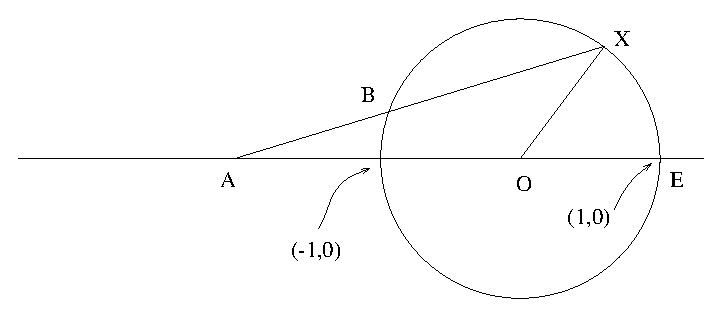
\includegraphics{figs/tri}
\caption{Trisection of the Angle with a marked ruler}
\end{figure}


Let $\theta$ be $\angle BAO$.
Then $\angle BOA = \theta$, and $\angle XBO = \angle BXO= 2\theta$

Since the sum of the internal angles of a triangle equals $\pi$
radians ($180$ degrees) we have $ \angle XBO + \angle BXO + \angle BOX
= \pi$, implying $4 \theta + \angle BOX = \pi$.  Also, we have that
$\angle AOB + \angle BOX + \angle XOE = \pi$, implying $\theta +\angle
BOX + \angle XOE = \pi$. Since both quantities are equal to $\pi$
we obtain

\[ 4 \theta + \angle BOX = \theta +\angle BOX + \angle XOE \]

From which

\[ 3 \theta = \angle XOE \]

follows. QED.



  \section{Which are the 23 Hilbert Problems?}
    The original was published in German in a couple of places.  A
translation was published by the AMS in 1902.
%
%From: Yannick.Saouter@irisa.fr (Saouter Yannick)
%Date: Wed, 6 Dec 1995 11:00:32 +0100
%

This article has been reprinted in 1976 by the American Mathematical
Society (see references).

The AMS Symposium mentioned at the end contains a series of papers on
the then-current state of most of the Problems, as well as the problems.

The URL contains the list of problems, and their current status:
\url{http://aleph0.clarku.edu/~djoyce/hilbert/problems.html}

% http://www.astro.virginia.edu/~eww6n/math/Hilbert'sProblems.html 



%Incidentally, the bibliography information above is taken from Yuri
%Matiyasevich's book ``Hilbert's Tenth Problem", published in 1993  by
%MIT Press.  The full bibliography is available via anonymous
%ftp from
%theory.lcs.mit.edu in the directory pub/hilbert10 (which also contains
%some other information about the book).

\book{Mathematical Developments Arising from Hilbert Problems,}
    {volume~28 of Proceedings of Symposia in Pure Mathematics,} {pages
    1--34, Providence, Rhode Island. American Mathematical Society,
    1976.}

\article{D. Hilbert.}  {Mathematical problems. Lecture delivered before
    the International Congress of Mathematicians at Paris in
    1900.}{Bulletin of the American Mathematical Society,}{8:437--479,
    1902.}
%%% Local Variables: 
%%% mode: latex
%%% TeX-master: "math-faq"
%%% End: 

  \section{Unsolved Problems}

\subsection{Does there exist a number that is perfect and odd?}

A given number is perfect if it is equal to the sum of all its proper
divisors. This question was first posed by Euclid in ancient Greece.
This question is still open.  Euler proved that if $N$ is an odd perfect
number, then in the prime power decomposition of $N$, exactly one
exponent is congruent to $1 \bmod 4$ and all the other exponents are
even. Furthermore, the prime occurring to an odd power must itself be
congruent to $1 \bmod 4$.  A sketch of the proof appears in Exercise 87,
page 203 of Underwood Dudley's Elementary Number Theory.  It has been
shown that there are no odd perfect numbers $< 10^{300}$.

\subsection{Collatz Problem}

\newcommand{\collatz}{\ensuremath{\mbox{\sc Collatz}}}
\begin{algorithm}[H]
  \caption{$\collatz(n)$}\label{alg:collatz}
  \begin{algorithmic}[1]

    \REQUIRE A natural number $m > 0$.

    \smallskip

    \STATE $n \leftarrow m$
    \REPEAT
        \IF{$n$ is odd}
            \STATE $n \leftarrow 3n + 1$
        \ELSE
            \STATE $n \leftarrow n/2$
        \ENDIF
    \UNTIL{$n = 1$}
  \end{algorithmic}
\end{algorithm}

\begin{conj}
  For all positive integers $m$, the Algorithm~\collatz{} terminates.
\end{conj}

The conjecture has been verified for all numbers up to $5.6 \times 10^{13}$.

\Ref

\book{Unsolved Problems in Number Theory.}{Richard K Guy.}{Springer,
  Problem E16.}

\book{Elementary Number Theory.}{Underwood Dudley.}{2nd ed.}

\article{G.T. Leavens and M. Vermeulen} {3x+1 search
  programs}{Comput. Math. Appl.}{vol. 24 n. 11 (1992), 79-99.}

\subsection{Goldbach's conjecture}

This conjecture claims that every even integer bigger equal to 4 is
expressible as the sum of two prime numbers.  It has been tested for all
values up to $4.10^{10}$ by Sinisalo.

%From: Saouter Yannick <Yannick.Saouter@irisa.fr>
%Date: Thu, 28 Nov 1996 09:09:45 +0100
%
%
%You precise that Goldbach's conjecture has been verified up to
%2*10^10. It is a work of te Riele and al. and there is a more
%recent work of Sinisalo:
%
%@article{Sinisalo,
%author= {{Sinisalo}, M.K.},
%title= {Checking the {G}oldbach Conjecture up to $4.10^{11}$},
%journal= {Math. Comp.},
%number={204},
%volume={61},
%pages={931-934},
%year= {1993}
%}

%From: David G Radcliffe <radcliff@csd.uwm.edu>
%Date: Mon, 27 Nov 1995 12:31:55 -0600 (CST)
%Conversely, it is known that Goldbach conjecture is true for all
%numbers larger than $e^{e^{16038}}$

\subsection{Twin primes conjecture}

There exist an infinite number of positive integers $p$ with $p$ and
$p+2$ both prime. See the largest known twin prime section. There are
some results on the estimated density of twin primes.
%%% Local Variables:
%%% mode: latex
%%% TeX-master: "math-faq"
%%% End:

\chapter{Mathematical Games}
  \section{The Monty Hall problem}

This problem has rapidly become part of the mathematical folklore.

The American Mathematical Monthly, in its issue of January 1992,
explains this problem carefully. The following are excerpted from
that article.

Problem:

A TV host shows you three numbered doors (all three equally likely),
one hiding a car and the other two hiding goats. You get to pick a door,
winning whatever is behind it. Regardless of the door you choose,
the host, who knows where the car is, then opens one of the other
two doors to reveal a goat, and invites you to switch your choice
if you so wish. Does switching increases your chances of winning
the car?

If the host always opens one of the two other doors, you should switch.
Notice that $1/3$ of the time you choose the right door (i.e. the one
with the car) and switching is wrong, while $2/3$ of the time you
choose the wrong door and switching gets you the car.

Thus the expected return of switching is $2/3$ which improves over
your original expected gain of $1/3$.

Even if the hosts offers you to switch only part of the time, it 
pays to switch.
Only in the case where we assume a malicious host (i.e. a host who
entices you to switch based in the knowledge that you have the right
door) would it pay not to switch.

There are several ways to convince yourself about why it pays to switch.
Here's one. You select a door. At this time assume the host asks
you if you want to switch {\bf before} he opens any doors. Even
though the odds that the door you selected is empty are high ($2/3$), there
is no advantage on switching as there are two doors, and you
don't know thich one to switch to. This means
the $2/3$ are evenly distributed, which as good as you are doing already.
However, once Monty opens one of the two doors you selected, the chances 
that you selected the right door are still $1/3$ and now you only have one door to
choose from if you switch. So it pays to switch.


\Ref

\article{L. Gillman}{The Car and the Goats}
        {American Mathematical Monthly,}{January 1992, pp. 3-7.}


\section{Master Mind}

    For the game of Master Mind it has been proven that no more than
    five moves are required in the worst case.

    One such algorithm was published in the Journal of Recreational
    Mathematics; in '70 or '71 (I think), which always solved the
    $4$ peg problem in $5$ moves. Knuth later published an algorithm which
    solves the problem in a shorter number of moves---on average---but can
    take six guesses on certain combinations.

    In 1994, Kenji Koyama and Tony W. Lai found, by exhaustive search
    that $5625/1296~=4.340$ is the optimal strategy in the expected
    case. This strategy may take six guesses in the worst case.
    A strategy that uses at most five guesses in the worst case
    is also shown. This strategy requires $5626/1296~=4.341$ guesses.


\Ref

    \article{Donald E. Knuth.}
            {The Computer as Master Mind.}
            {J. Recreational Mathematics,}
            { 9 (1976-77), 1-6.}

    \article{Kenji Koyama, Tony W. Lai.}
            {An optimal Mastermind Strategy.}
            {J. Recreational Mathematics,}
            {Vol. 25, Number 3, pp.251-256.}

\chapter{Axiom of Choice and Continuum Hypothesis}
  \section{The Axiom of Choice}

There are several equivalent formulations:

\begin{itemize}

  \item The Cartesian product of nonempty sets is nonempty, even if the
  product is of an infinite family of sets.

  \item Given any set $S$ of mutually disjoint nonempty sets, there is a
  set $C$ containing a single member from each element of $S$.  $C$ can
  thus be thought of as the result of ``choosing'' a representative from
  each set in $S$. Hence the name.
\end{itemize}

\subsection{Relevance of the Axiom of Choice}
THE AXIOM OF CHOICE

There are many equivalent statements of the Axiom of Choice.  The
following version gave rise to its name:
\begin{quote}
  For any set $X$ there is a function $f$, with domain $X\backslash{0}$,
  so that $f(x)$ is a member of $x$ for every nonempty $x$ in $X$.
\end{quote}

Such an $f$ is called a ``choice function'' on $X$.  [Note that
$X\backslash {0}$ means $X$ with the empty set removed.  Also note that
in Zermelo-Fraenkel set theory all mathematical objects are sets so each
member of $X$ is itself a set.]

The Axiom of Choice (AC) is one of the most discussed axioms of
mathematics, perhaps second only to Euclid's parallel postulate.  The
axioms of set theory provide a foundation for modern mathematics in the
same way that Euclid's five postulates provided a foundation for
Euclidean geometry, and the questions surrounding AC are the same as the
questions that surrounded Euclid's Parallel Postulate:

\begin{enumerate}
  \item Can it be derived from the other axioms?
  \item Is it consistent with the other axioms?
  \item Should we accept it as an axiom?
\end{enumerate}

For many sets, including any finite set, the first six axioms of set
theory (abbreviated ZF) are enough to guarantee the existence of a
choice function but there do exist sets for which AC is {\em required}
to show the existence of a choice function.  The existence of such sets
was proved in 1963 by Paul Cohen.  This means that AC cannot be derived
from the other six axioms; in other words ``AC is independent of ZF.''
This answers question [1] posed above.

The question of whether AC is consistent with the other axioms (question
[2] above) was answered by Goedel in 1938.  Goedel showed that if the
other axioms are consistent then AC is consistent with them.  This is a
``relative consistency'' proof which is the best we can hope for because
of Goedel's Second Incompleteness Theorem.

The third question, ``Should we accept it as an axiom?'', moves us into
the realm of philosophy.  Today there are three major schools of thought
concerning the use of AC:

\begin{enumerate}
  \item Accept it as an axiom and use it without hesitation.
  \item Accept it as an axiom but use it only when you cannot find a
  proof without it.
  \item AC is unacceptable.
\end{enumerate}

Most mathematicians today belong to school A.  Mathematicians who are in
school B are usually there because of a belief in Occam's Razor (use as
few assumptions as possible when explaining something) or an interest in
metamathematics.  There are a growing number of people moving to school
C, especially computer scientists who work on automated reasoning using
constructive type theories.

Underlying the schools of thought about the use of AC are views about
truth and the nature of mathematical objects.  Three major views are
platonism, constructivism, and formalism.

\subsubsection{Platonism}

A platonist believes that mathematical objects exist independent of the
human mind, and a mathematical statement, such as AC, is objectively
either true or false.  A platonist accepts AC only if it is objectively
true, and probably falls into school A or C depending on her belief.  If
she isn't sure about AC's truth then she may be in school B so that once
she finds out the truth about AC she will know which theorems are true.

\subsubsection{Constructivism}

A constructivist believes that the only acceptable mathematical objects
are ones that can be constructed by the human mind, and the only
acceptable proofs are constructive proofs.  Since AC gives no method for
constructing a choice set constructivists belong to school C.

\subsubsection{Formalism}

A formalist believes that mathematics is strictly symbol manipulation
and any consistent theory is reasonable to study.  For a formalist the
notion of truth is confined to the context of mathematical models, e.g.,
a formalist would say ``The parallel postulate is false in Riemannian
geometry.'' but she wouldn't say ``The parallel postulate is false.''  A
formalist will probably not allign herself with any school.  She will
comfortably switch between A, B, and C depending on her current
interests.


So: Should you accept the Axiom of Choice?  Here are some arguments for
and against it.

\subsubsection{Against}

\begin{itemize}
  \item It's not as simple, aesthetically pleasing, and intuitive as the
  other axioms.
  \item It is equivalent to many statements which are not intuitive such
  as ``Every set can be well ordered.''  How, for example, would you
  well order the reals?
  \item With it you can derive non-intuitive results, such as the
  existence of a discontinuous additive function, the existence of a
  non-measurable set of reals, and the Banach-Tarski Paradox (see the
  next section of the sci.math FAQ).
  \item It is nonconstructive---it conjures up a set without providing
  any sort of procedure for its construction.
\end{itemize}

\subsubsection{For}

The acceptance of AC is based on the belief that our intuition about
finite sets can be extended to infinite sets.  The main argument for
accepting it is that it is useful.  Many important, intuitively
plausible theorems are equivalent to it or depend on it.  For example
these statements are equivalent to AC:
\begin{itemize}
  \item Every vector space has a basis.
  \item Trichotomy of Cardinals: For any cardinals $k$ and $l$, either
  $k<l$ or $k=l$ or $k>l$.
  \item Tychonoff's Theorem: The product of compact spaces is compact in
  the product topology.
  \item Zorn's Lemma: Every nonempty partially ordered set P in which
  each chain has an upper bound in P has a maximal element.
\end{itemize}

And these statements depend on AC (i.e., they cannot be proved in ZF
without AC):

\begin{itemize}
  \item The union of countably many countable sets is countable.
  \item Every infinite set has a denumerable subset.
  \item The Loewenheim-Skolem Theorem: Any first-order theory which has
  a model has a denumerable model.
  \item The Baire Category Theorem: The reals are not the union of
  countably many nowhere dense sets (i.e., the reals are not meager).
  \item The Ultrafilter Theorem: Every Boolean algebra has an
  ultrafilter on it.
\end{itemize}

\subsubsection{Alternatives to AC}

\begin{itemize}
  \item Accept only a weak form of AC such as the Denumerable Axiom of
  Choice (every denumerable set has a choice function) or the Axiom of
  Dependent Choice.
  \item Accept an axiom that implies AC such as the Axiom of
  Constructibility ($V=L$) or the Generalized Continuum Hypothesis
  (GCH).
  \item Adopt AC as a logical axiom (Hilbert suggested this with his
  epsilon axiom).  If set theory is done in such a logical formal system
  the Axiom of Choice will be a theorem.
  \item Accept a contradictory axiom such as the Axiom of Determinacy.
  \item Use a completely different framework for mathematics such as
  Category Theory.  Note that within the framework of Category Theory
  Tychonoff's Theorem can be proved without AC (Johnstone, 1981).
\end{itemize}

\subsubsection{Test Yourself: When is AC necessary?}

If you are working in Zermelo-Fraenkel set theory without the Axiom of
Choice, can you choose an element from...
\begin{enumerate}
  \item a finite set?
  \item an infinite set?
  \item each member of an infinite set of singletons (i.e., one-element
  sets)?
  \item each member of an infinite set of pairs of shoes?
  \item each member of inifinite set of pairs of socks?
  \item each member of a finite set of sets if each of the members is
  infinite?
  \item each member of an infinite set of sets if each of the members is
  infinite?
  \item each member of a denumerable set of sets if each of the members
  is infinite?
  \item each member of an infinite set of sets of rationals?
  \item each member of a denumerable set of sets if each of the members
  is denumberable?
  \item each member of an infinite set of sets if each of the members is
  finite?
  \item each member of an infinite set of finite sets of reals?
  \item each member of an infinite set of sets of reals?
  \item each member of an infinite set of two-element sets whose members
  are sets of reals?
\end{enumerate}
The answers to these questions with explanations are accessible through
\url{http://www.jazzie.com/ii/math/index.html}.

\Ref

Benacerraf, Paul and Putnam, Hilary.  ``Philosophy of Mathematics:
Selected Readings'', 2nd edition. Cambridge University Press, 1983.

Dauben, Joseph Warren.  ``Georg Cantor: His Mathematics and Philosophy
of the Infinite.''  Princeton University Press, 1979.

A. Fraenkel, Y.  Bar-Hillel, and A. Levy with van Dalen, Dirk.
``Foundations of Set Theory,'' Second Revised Edition.  North-Holland,
1973.

Johnstone, Peter T.  ``Tychonoff's Theorem without the Axiom of
Choice.''  Fundamenta Mathematica 113: 21-35, 1981.

Leisenring, Albert C.  ``Mathematical Logic and Hilbert's
Epsilon-Symbol.''  Gordon and Breach, 1969.

Maddy, ``Believing the Axioms, I'', J. Symb. Logic, v. 53, no. 2, June
1988, pp. 490-500, and ``Believing the Axioms II'' in v.53, no. 3.

Moore, Gregory H.  ``Zermelo's Axiom of Choice: Its Origins,
Development, and Influence.''  Springer-Verlag, 1982.

Rubin, Herman and Rubin, Jean E.  ``Equivalents of the Axiom of Choice
II.''  North-Holland, 1985.

This section of the FAQ is Copyright © 1994 Nancy McGough.  Send
comments and or corrections relating to this part to
\url{nancym@ii.com}.  The most up to date version of this section of the
\href{news://sci.math}{\texttt{sci.math}} FAQ is accesible through
\url{http://www.jazzie.com/ii/math/index.html}.
%%% Local Variables:
%%% mode: latex
%%% TeX-master: "math-faq"
%%% End:

  \section{Cutting a sphere into pieces of larger volume}


Is it possible to cut a sphere into a finite number of pieces and
reassemble into a solid of twice the volume?

This question has many variants and it is best answered explicitly.

Given two polygons of the same area, is it always possible to dissect
one into a finite number of pieces which can be reassembled into a
replica of the other?

Dissection theory is extensive.  In such questions one needs to specify

\begin{itemize}
  \item What is a ``piece''?  (polygon?  Topological disk?  Borel-set?
  Lebesgue-measurable set?  Arbitrary?)

  \item How many pieces are permitted (finitely many? countably?
  uncountably?)

  \item What motions are allowed in ``reassembling'' (translations?
  rotations?  orientation-reversing maps?  isometries?  affine maps?
  homotheties?  arbitrary continuous images?  etc.)

  \item How the pieces are permitted to be glued together.  The simplest
  notion is that they must be disjoint.  If the pieces are polygons [or
  any piece with a nice boundary] you can permit them to be glued along
  their boundaries, ie the interiors of the pieces disjoint, and their
  union is the desired figure.
\end{itemize}

Some dissection results

\begin{itemize}
  \item We are permitted to cut into finitely many polygons, to
  translate and rotate the pieces, and to glue along boundaries; then
  yes, any two equal-area polygons are equi-decomposable.

  This theorem was proven by Bolyai and Gerwien independently, and has
  undoubtedly been independently rediscovered many times.  I would not
  be surprised if the Greeks knew this.

  The Hadwiger-Glur theorem implies that any two equal-area polygons are
  equi-decomposable using only translations and rotations by $180$
  degrees.

  \item
  \begin{teo}[Hadwiger-Glur, 1951]
    Two equal-area polygons $P$,$Q$ are equi-decomposable by
    translations only, iff we have equality of these two functions:
    $\phi_P() = \phi_Q()$
  \end{teo}
  Here, for each direction $v$ (ie, each vector on the unit circle in
  the plane), let $\phi_P(v)$ be the sum of the lengths of the edges of
  $P$ which are perpendicular to $v$, where for such an edge, its length
  is positive if $v$ is an outward normal to the edge and is negative if
  $v$ is an inward normal to the edge.


  \item In dimension 3, the famous ``Hilbert's third problem'' is:
  \begin{quote}
    If $P$ and $Q$ are two polyhedra of equal volume, are they
    equi-decomposable by means of translations and rotations, by cutting
    into finitely many sub-polyhedra, and gluing along boundaries?
  \end{quote}

  The answer is {\bf no} and was proven by Dehn in 1900, just a few
  months after the problem was posed. (Ueber raumgleiche polyeder,
  Goettinger Nachrichten 1900, 345-354). It was the first of Hilbert's
  problems to be solved. The proof is nontrivial but does not use the
  axiom of choice.

  \Ref

  \book{Hilbert's Third Problem.}{V.G. Boltianskii.}{Wiley 1978.}


  \item Using the axiom of choice on non-countable sets, you can prove
  that a solid sphere can be dissected into a finite number of pieces
  that can be reassembled to two solid spheres, each of same volume of
  the original. No more than nine pieces are needed.

  The minimum possible number of pieces is five.  (It's quite easy to
  show that four will not suffice).  There is a particular dissection in
  which one of the five pieces is the single center point of the
  original sphere, and the other four pieces $A$, $A^\prime$, $B$,
  $B^\prime$ are such that $A$ is congruent to $A^\prime$ and $B$ is
  congruent to $B^\prime$.  [See Wagon's book].

  This construction is known as the {\em Banach-Tarski paradox} or the
  {\em Banach-Tarski-Hausdorff} paradox (Hausdorff did an early version
  of it).  The ``pieces'' here are non-measurable sets, and they are
  assembled disjointly (they are not glued together along a boundary,
  unlike the situation in Bolyai's thm.)  An excellent book on
  Banach-Tarski is:


  \book{The Banach-Tarski Paradox.}{Stan Wagon.}{Cambridge University
    Press, 985}

  \article{Robert M. French.}{The Banach-Tarski theorem.}{The
    Mathematical Intelligencer,}{10 (1988) 21-28.}


  The pieces are not (Lebesgue) measurable, since measure is preserved
  by rigid motion. Since the pieces are non-measurable, they do not have
  reasonable boundaries. For example, it is likely that each piece's
  topological-boundary is the entire ball.

  The full Banach-Tarski paradox is stronger than just doubling the
  ball.  It states:

  \item Any two bounded subsets (of $3$-space) with non-empty interior,
  are equi-decomposable by translations and rotations.

  This is usually illustrated by observing that a pea can be cut up into
  finitely pieces and reassembled into the Earth.

  The easiest decomposition ``paradox'' was observed first by Hausdorff:

  \item The unit interval can be cut up into countably many pieces
  which, by translation only, can be reassembled into the interval of
  length 2.

  This result is, nowadays, trivial, and is the standard example of a
  non-measurable set, taught in a beginning graduate class on measure
  theory.
  \item
  \begin{teo}
    There is a finite collection of disjoint open sets in the unit cube
    in $R^3$ which can be moved by isometries to a finite collection of
    disjoint open sets whose union is dense in the cube of size 2 in
    $R^3$.
  \end{teo}
  This result is by Foreman and Dougherty.

%Jorge Stolfi
%stolfi@dcc.unicamp.br

  \item A square {\bf cannot} be rearranged into a disk, if one is
  allowed finitely many pieces with analytic boundaries, glued at edges.
  \item A square can be rearranged into a disk, with translations only,
  if one is allowed to use finitely many pieces with unconstrained shape
  (not necessarily connected), and disjoint assembly.
\end{itemize}

\Ref

\article{Boltyanskii.}{Equivalent and equidecomposable figures.}  {in
  Topics in Mathematics published by D.C. HEATH AND CO., Boston.}{}

\article{Dubins, Hirsch and ?}{Scissor Congruence}{American Mathematical
  Monthly.}{}

``Banach and Tarski had hoped that the physical absurdity of this
theorem would encourage mathematicians to discard AC. They were dismayed
when the response of the math community was `Isn't AC great?  How else
could we get such counterintuitive results?'{}''

  \section{The Continuum Hypothesis}
    A basic reference is Godel's ``What is Cantor's Continuum Problem?'',
from 1947 with a 1963 supplement, reprinted in Benacerraf and Putnam's
collection Philosophy of Mathematics.  This outlines Godel's generally
anti-CH views, giving some ``implausible'' consequences of CH.

\begin{quote}
  ``I believe that adding up all that has been said one has good reason
  to suspect that the role of the continuum problem in set theory will
  be to lead to the discovery of new axioms which will make it possible
  to disprove Cantor's conjecture.''
\end{quote}

At one stage he believed he had a proof that $C = \aleph_2$ from some
new axioms, but this turned out to be fallacious.  (See Ellentuck,
``Godel's Square Axioms for the Continuum'', Mathematische Annalen
1975.)

Maddy's ``Believing the Axioms'', Journal of Symbolic Logic 1988 (in 2
parts) is an extremely interesting paper and a lot of fun to read.  A
bonus is that it gives a non-set-theorist who knows the basics a good
feeling for a lot of issues in contemporary set theory.

Most of the first part is devoted to ``plausible arguments'' for or
against CH: how it stands relative to both other possible axioms and to
various set-theoretic ``rules of thumb''.  One gets the feeling that the
weight of the arguments is against CH, although Maddy says that many
``younger members'' of the set-theoretic community are becoming more
sympathetic to CH than their elders.  There's far too much here for me
to be able to go into it in much detail.

Some highlights from Maddy's discussion, also incorporating a few things
that other people sent me:

\begin{enumerate}
  \item Cantor's reasons for believing CH aren't all that persuasive today.

  \item Godel's proof of the consistency of CH shows that CH follows
  from ZFC plus the Axiom of Constructibility ($V=L$, roughly that the
  set-theoretic universe = the constructible universe).  However, most
  set-theorists seem to find Constructiblity implausible and much too
  restrictive.  It's an example of a ``minimizing'' principle, which
  tends to cut down on the number of sets admitted to one's universe.
  Apparently ``maximizing'' principles meet with much more sympathy from
  set theorists.  Such principles are more compatible with $\neg$CH than
  with CH.

  \item If GCH is true, this implies that $\aleph_0$ has certain unique
  properties: e.g. that it's that cardinal before which GCH is false and
  after which it is true.  Some would like to believe that the
  set-theoretic universe is more ``uniform'' (homogeneous) than that,
  without this kind of singular occurrence.  Such a ``uniformity''
  principle tends to imply $\neg$GCH.

  \item Most of those who disbelieve CH think that the continuum is
  likely to have very large cardinality, rather than $\aleph_2$ (as
  Godel seems to have suggested).  Even Cohen, a professed formalist,
  argues that the power set operation is a strong operation that should
  yield sets much larger than those reached quickly by stepping forward
  through the ordinals:

  \begin{quote}
    ``This point of view regards C as an incredibly rich set given to us
    by a bold new axiom, which can never be approached by any piecemeal
    process of construction.''
  \end{quote}

  \item There are also a few arguments in favour of CH, e.g. there's an
  argument that $\neg$CH is restrictive (in the sense of (2) above).
  Also, CH is much easier to force (Cohen's method) than $\neg$CH.  And
  CH is much more likely to settle various outstanding results than is
  $\neg$CH, which tends to be neutral on these results.

  \item Most large cardinal axioms (asserting the existence of cardinals
  with various properties of hugeness: these are usually derived either
  from considering the hugeness of $\aleph_0$ compared to the finite
  cardinals and applying uniformity, or from considering the hugeness of
  V (the set-theoretic universe) relative to all sets and applying
  ``reflection'') don't seem to settle CH one way or the other.

  \item Various other axioms have some bearing.  Axioms of determinacy
  restrict the class of sets of reals that might be counterexamples to
  CH.  Various forcing axioms (e.g. Martin's axiom), which are
  ``maximality'' principles (in the sense of (2) above), imply $\neg$CH.
  The strongest (Martin's maximum) implies that $C = \aleph_2$.  Of
  course the ``truth'' or otherwise of all these axioms is
  controversial.

  \item Freiling's principle about ``throwing darts at the real line''
  is a seemingly very plausible principle, not involving large cardinals
  at all, from which $\neg$CH immediately follows.  Freiling's paper
  (JSL 1986) is a good read.  More on this at the end of this message.
\end{enumerate}

Of course we have conspicuously avoided saying anything about whether
it's even reasonable to suppose that CH has a determinate truth-value.
Formalists will argue that we may choose to make it come out whichever
way we want, depending on the system we work in.  On the other hand, the
mere fact of its independence from ZFC shouldn't immediately lead us to
this conclusion -- this would be assigning ZFC a privileged status which
it hasn't necessarily earned.  Indeed, Maddy points out that various
axioms within ZFC (notably the Axiom of Choice, and also Replacement)
were adopted for extrinsic reasons (e.g. ``usefulness'') as well as for
``intrinsic'' reasons (e.g. ``intuitiveness'').  Further axioms, from
which CH might be settled, might well be adopted for such reasons.

One set-theorist correspondent said that set-theorists themselves are
very loathe to talk about ``truth'' or ``falsity'' of such claims.
(They're prepared to concede that $2+2=4$ is true, but as soon as you
move beyond the integers trouble starts.  e.g. most were wary even of
suggesting that the Riemann Hypothesis necessarily has a determinate
truth-value.)  On the other hand, Maddy's contemporaries discussed in
her paper seemed quite happy to speculate about the ``truth'' or
``falsity'' of CH.

The integers are not only a bedrock, but also any finite number of power
sets seem to be quite natural Intuitively are also natural which would
point towards the fact that CH may be determinate one way or the other.
As one correspondent suggested, the question of the determinateness of
CH is perhaps the single best way to separate the Platonists from the
formalists.

And is it true or false?  Well, CH is somewhat intuitively plausible.
But after reading all this, it does seem that the weight of evidence
tend to point the other way.

The following is from Bill Allen on Freiling's Axiom of Symmetry.  This
is a good one to run your intuitions by.

\begin{quote}
  Let $A$ be the set of functions mapping Real Numbers into countable
  sets of Real Numbers.  Given a function $f$ in $A$, and some arbitrary
  real numbers $x$ and $y$, we see that $x$ is in $f(y)$ with
  probability 0, i.e. $x$ is not in $f(y)$ with probability 1.
  Similarly, $y$ is not in $f(x)$ with probability 1.  Let AX be the
  axiom which states

  ``for every $f$ in $A$, there exist $x$ and $y$ such that $x$ is not
  in $f(y)$ and $y$ is not in $f(x)$''

  The intuitive justification for AX is that we can find the $x$ and $y$
  by choosing them at random.

  In ZFC, AX = not CH.

  proof:

  If CH holds, then well-order $R$ as $r_0, r_1, .... , r_x, ...$ with
  $x < \aleph_1$.  Define $f(r_x)$ as $\{r_y : y \leq x\}$.  Then $f$ is
  a function which witnesses the falsity of AX.

  If CH fails, then let $f$ be some member of $A$.  Let $Y$ be a subset
  of $R$ of cardinality $\aleph_1$.  Then $Y$ is a proper subset.  Let
  $X$ be the union of all the sets $f(y)$ with $y$ in $Y$, together with
  $Y$.  Then, as $X$ is an $\aleph_1$ union of countable sets, together
  with a single $\aleph_1$ size set $Y$, the cardinality of $X$ is also
  $\aleph_1$, so $X$ is not all of $R$.  Let a be in $R \ X$, so that a
  is not in $f(y)$ for any $y$ in $Y$.  Since $f(a)$ is countable, there
  has to be some $b$ in $Y$ such that $b$ is not in $f(a)$.  Thus we
  have shown that there must exist $a$ and $b$ such that $a$ is not in
  $f(b)$ and $b$ is not in $f(a)$.  So AX holds.
\end{quote}

Freiling's proof, does not invoke large cardinals or intense infinitary
combinatorics to make the point that CH implies counter-intuitive
propositions.  Freiling has also pointed out that the natural extension
of AX is AXL (notation mine), where AXL is AX with the notion of
countable replaced by Lebesgue Measure zero.  Freiling has established
some interesting Fubini-type theorems using AXL.

See ``Axioms of Symmetry: Throwing Darts at the Real Line'', by
Freiling, Journal of Symbolic Logic, 51, pages 190-200.  An extension of
this work appears in ``Some properties of large filters'', by Freiling
and Payne, in the JSL, LIII, pages 1027-1035.

The section above was excerpted from a posting from David Chalmers, of
Indiana University.

See also

Nancy McGough's *Continuum Hypothesis article* or its *mirror*.

\url{http://www.jazzie.com/ii/math/ch/}

\url{http://www.best.com/~ii/math/ch/}
%%% Local Variables: 
%%% mode: latex
%%% TeX-master: "math-faq"
%%% End: 

\chapter{Formulas of General Interest}
  \section{How to determine the day of the week, given the month,
             day and year}
     First a brief explanation: In the Gregorian Calendar, over a period
    of four hundred years, there are 97 leap years and 303 normal years.
    Each normal year, the day of January 1 advances by one; for each leap
    year it advances by two.

     \[   303 + 97 + 97 = 497 = 7 * 71 \]

    As a result, January 1 year $N$ occurs on the same day of the week as
    January 1 year $N + 400$.  Because the leap year pattern also recurs
    with a four hundred year cycle, a simple table of four hundred
    elements, and single modulus, suffices to determine the day of the
    week (in the Gregorian Calendar), and does it much faster than all the
    other algorithms proposed.  Also, each element takes (in principle)
    only three bits; the entire table thus takes only 1200 bits; 
    %Date: Mon, 20 Nov 1995 08:51:23 +0100
    %From: Juergen Weinelt <rzuw039@rz.uni-wuerzburg.de>
    %1200/8=150
    %
    %or 300 bytes; 
    on many computers this will be less than the instructions to do
    all the complicated calculations proposed for the other algorithms.

    Incidental note: Because 7 does not divide 400, January 1 occurs more
    frequently on some days than others!  Trick your friends!  In a cycle
    of 400 years, January 1 and March 1 occur on the following days with
    the following frequencies:

\begin{verbatim}
           Sun      Mon     Tue     Wed     Thu     Fri     Sat
    Jan 1: 58       56      58      57      57      58      56
    Mar 1: 58       56      58      56      58      57      57
\end{verbatim}

    Of interest is that (contrary to most initial guesses) the occurrence
    is not maximally flat.

    % I saw the article in the Gazette. I remember having seen this 
    % result before. AL-O
    % Also ray johnstone <ray@iinet.com.au> pointed it out on Tue, 11 Apr 1995

    In the Mathematical Gazette, vol. 53,, pp.127-129, it is shown that 
    the 13th of the month is more likely to be a Friday than any other
    day.The author is a 13 year old S.R.Baxter.


    The Gregorian calendar was introduced in 1582 in parts of Europe; it was
    adopted in 1752 in Great Britain and its colonies, and on various dates
    in other countries.  It replaced the Julian Calendar which has a four-year
    cycle of leap years; after four years January 1 has advanced by five days.
    Since 5 is relatively prime to 7, a table of $4 * 7 = 28$ elements is
    necessary for the Julian Calendar.


    There is still a 3 day over 10,000 years error which the Gregorian calendar
    does not take into account.  At some time such a correction will have
    to be done but your software will probably not last that long!

    Here is a standard method suitable for mental computation:


\begin{enumerate}
        \item Take the last two digits of the year.
        \item Divide by 4, discarding any fraction.
        \item Add the day of the month.
        \item Add the month's key value: JFM AMJ JAS OND
                                         144 025 036 146
        \item Subtract 1 for January or February of a leap year.
        \item For a Gregorian date, add 0 for 1900's, 6 for 2000's,
             4 for 1700's,
           2 for 1800's; for other years, add or subtract multiples of 400.
        \item For a Julian date, add 1 for 1700's, and 1 for every additional
           century you go back.
        \item Add the last two digits of the year.
        \item Divide by 7 and take the remainder.
\end{enumerate}

        Now 1 is Sunday, the first day of the week, 2 is Monday, and so on.

    The following formula, which is for the Gregorian calendar only, may be
    more convenient for computer programming.  Note that in some programming
    languages the remainder operation can yield a negative result if given
    a negative operand, so mod 7 may not translate to a simple remainder.
       \[ W = (k + \lfloor 2.6m - 0.2\rfloor - 2C + Y + \lfloor Y/4
\rfloor + \lfloor C/4\rfloor) mod 7 \]
           where $\lfloor\ \rfloor$  denotes the integer floor function,\\
           $k$ is day (1 to 31)\\
           $m$ is month (1 = March, ..., 10 = December, 11 = Jan, 12 = Feb)
                         Treat Jan \& Feb as months of the preceding year\\
           $C$ is century (1987 has $C$ = 19)\\
           $Y$ is year    (1987 has $Y$ = 87 except $Y$ = 86 for Jan \& Feb)\\
           $W$ is week day (0 = Sunday, ..., 6 = Saturday)\\

    Here the century and 400 year corrections are built into the formula.
    The $\lfloor 2.6m-0.2\rfloor$ term relates to the repetitive pattern that the 30-day
    months show when March is taken as the first month.

The following short C program works for a restricted range, it returns 0 for
Monday, 1 for Tuesday, etc.

\begin{verbatim}
dow(m,d,y){y-=m<3;return(y+y/4-y/100+y/400+"-bed=pen+mad."[m]+d)%7;}
\end{verbatim}

The program appeared  was posted by
\url{sakamoto@sm.sony.co.jp} (Tomohiko Sakamoto) on comp.lang.c on March
10th, 1993.

A good mnemonic rule to help on the computation of the day of the week is
as follows. In any given year the following days come on
the same day of the week:

\begin{verbatim}
4/4
6/6
8/8
10/10
12/12
\end{verbatim}

\noindent to remember the next four, remember that I work from 9--5 at a 7--11 so

\begin{verbatim}
9/5
5/9
7/11
11/7
\end{verbatim}

\noindent and the last day of Feb.

``In 1995 they come on Tuesday. Every year this advances one other than
leap-years which advance 2. Therefore for 1996 the day will be
Thursday, and for 1997 it will be Friday. Therefore ordinarily every 4
years it advances 5 days. There is a minor correction for the century
since the century is a leap year iff the century is divisible by 4.
Therefore 2000 is a leap year, but 1900, 1800, and 1700 were not.''

Even ignoring the pattern over for a period of years this is still
useful since you can generally figure out what day of the week a given
date is on faster than someone else can look it up with a calender if
the calender is not right there. (A useful skill that.)


    \Ref

    \book{Winning Ways for your mathematical plays.}{Elwyn
R. Berlekamp, John H. Conway, and Richard K. Guy}
    {London ; Toronto : Academic Press, 1982.}

    \book{Mathematical Carnival.}{Martin Gardner.}{New York : Knopf, c1975.}

    \book{Elementary Number Theory and its applications.}{Kenneth Rosen.}
    {Reading, Mass. ; Don Mills, Ont. : Addison-Wesley Pub. Co., c1993. p. 156.}


    \article{Michael Keith and Tom Craver.}{The Ultimate Perpetual Calendar?}
    {Journal of Recreational Mathematics,}{22:4, pp. 280-282, 19}

   \section{Symbolic Computation Packages}

This is not a comprehensive list. There are other Computer Algebra
packages available that may better suit your needs. There is an
Available Packages listing maintained at UC Berkeley.  (The list can be
obtained from \href{ftp://math.berkeley.edu/} via anonymous ftp).

%From: Xah Lee <xah@best.com>    
%Date: Mon, 9 Jun 1997 14:38:41 -0700 (PDT)                       
The \href{http://symbolicnet.mcs.kent.edu/}{Symbolic Computation
  Network} contains lots of useful information.

\begin{verbatim}
A: Maple
        Purpose: Symbolic and numeric computation, mathematical
        programming, and mathematical visualization.
        Contact: Waterloo Maple Software,
        450 Phillip Street
        Waterloo, Ontario
        N2L 5J2
        Phone (519)747-2373
        FAX   (519)747-5284
        email:  info@maplesoft.on.ca

A: DOE-Macsyma
        Purpose: Symbolic and mathematical manipulations.
        Contact: National Energy Software Center
        Argonne National Laboratory 9700 South Cass Avenue
        Argonne, Illinois 60439
        Phone: (708) 972-7250

A: Pari
        Purpose: Number-theoretic computations and simple numerical
        analysis.
        Available for most 32-bit machines, including 386+387 and 486.
        This is a copyrighted but free package, available by ftp from
        math.ucla.edu (128.97.4.254) and ftp.inria.fr (128.93.1.26).
        Contact: questions about pari can be sent to pari@math.u-bordeaux.fr
        and for the Macintosh versions to bernardi@mathp7.jussieu.fr

A: Mathematica
        Purpose: Mathematical computation and visualization,
        symbolic programming.
        Contact: Wolfram Research, Inc.
        100 Trade Center Drive Champaign,
        IL 61820-7237
        Phone: 1-800-441-MATH

A: Macsyma
        Purpose: Symbolic numerical and graphical mathematics.
        Contact: Macsyma Inc.
        20 Academy Street
        Arlington, MA 02174
        tel: 617-646-4550
        fax: 617-646-3161
        email: info-macsyma@macsyma.com

A: Matlab
        Purpose: `matrix laboratory' for tasks involving
        matrices, graphics and general numerical computation.
        Contact: The MathWorks, Inc.
        21 Prime Park Way
        Natick, MA 01760
        508-653-1415
        info@mathworks.com

A: Cayley/Magma
        A: Cayley/Magma
        Cayley is no longer being licenced or supported.
        It has been superseded by a new and more powerful system
        called Magma.
        Purpose: Computation in algebraic, geometric and
        combinatorial structures such as groups, rings, fields,
        algebras, modules, graphs and codes.
        Available for: SUN 3, SUN 4, SUN 10 (SUNOS 4.x and Solaris 2)
        DECstation (Ultrix), DEC Alpha (OSF/1), IBM RS6000 (AIX),
        HP9000/700 (HP-UX), Apollo M680x0, SGI, 486/Pentium (MS-DOS).
        Contact: Computational Algebra Group
        School of Mathematics and Statistics
        University of Sydney
        NSW 2006
        Australia
        Phone:  +61 2 351 3338
        Fax: +61 2 351 4534
        URL: http://www.maths.usyd.edu.au:8000/comp/magma/Overview.html
        magma@maths.su.oz.au

A: Axiom
        Purpose: Symbolic programming, symbolic and numeric computation,
                 mathematical visualisation.
        Contact: The Numerical Algorithms Group Ltd
        Wilkinson House
        Jordan Hill Road
        Oxford
        OX2 8DR
        UK
        email:  infodesk@nag.co.uk
        Phone: +44 1865 311744
        Fax:   +44 1865 311755
\end{verbatim}

  \section{Formula for the Surface Area of a sphere in Euclidean $N$-Space}
    
This is equivalent to the volume of the $N$-1
    solid which comprises the boundary of an $N$-Sphere.

The volume of a ball is the easiest formula to remember:  It's 
$r^N \frac{\pi^{N/2}}{(N/2)!}$.
     The only hard part is taking the factorial
    of a half-integer.  The real definition is that $x! = \Gamma(x+1)$, but
    if you want a formula, it's:

    \[(1/2+n)! = \sqrt{\pi} \frac{(2n+2)!}{(n+1)!4^{n+1}}\]
    To get the surface area, you just differentiate to get
    $N\frac{\pi^{N/2}}{(N/2)!}r^{N-1}$.

    There is a clever way to obtain this formula using Gaussian
    integrals. First, we note that the integral over the line of
    $e^{-x^2}$ is $\sqrt{\pi}$.  Therefore the integral over $N$-space of
    $e^{-x_1^2-x_2^2-...-x_N^2}$ is $\sqrt{\pi}^n$.  Now we change to
    spherical coordinates.  We get the integral from 0 to infinity
    of $Vr^{N-1}e^{-r^2}$, where $V$ is the surface volume of a sphere.
    Integrate by parts repeatedly to get the desired formula.

    It is possible to derive the volume of the sphere from ``first 
    principles''.



  \section{Formula to compute compound interest.}
    Here's a formula which can be used in 123, Excel, Wings and Dynaplan:

\begin{verbatim}
     ------- Input this data -------------------------------
     principal amount = E9                  ( in dollars )
     Amortization Period = d10              ( in years ie 6 mon = .5 )
     Payments / year = D11                  ( 12 = monthly, 52 = weekly )
     Published Interest rate = D12          ( ie 9 % = 0.09 )
     Times per year Int calculated = d13    ( CDN mortgage use 2
                                         US mortgage use 12
                                         all other loans use 12 )
     ----- Calculate the proper rate of interest -----------

     e14 = Effective annual rate = EXP(D13*LN(1+(D12/D13)))-1
     e15 = Interest rate per payment = (EXP(LN(E14+1)/(D10*D11))-1)*D10*D11

     e17 = Payments = APMT(E9,E15/D11,D10*D11) ( both these functions are
                    = PMT (E9,E15/D11,D10*D11) ( identical,diff spreadsheet)
           APMT( principal amount,interest rate per period,# periods )
           ( this is a standard function on any true commercial spreadsheet)

           OR use the following if done using a calculator
         = Payments = P*I/[1-(I+1)^-T]
                    = E9*(E15/D11)/(1-((E15/D11) +1)**(-1*D10*D11))

     Total interest cost = E17*D10*D11-E9

     -- Use these formulas if you wish to generate an amortization table --
     always add up to 'Payments (e17)'
     Interest per payment  = current balance * ( E15 / D11 )
     Principal per payment = current balance - Interest per payment
     new current balance   = current balance - Principal per payment -
                             (extra payment)

        keep repeating until 'new current balance' = 0

\end{verbatim}

Derivation of Compound Interest Rate Formula

Suppose you deposited a fixed payment into an interest bearing account
at regular intervals, say monthly, at the end of each month.  How much
money would there be in the account at the end of the nth month (at
which point you've made $n$ payments)?

\noindent Let $i$ be the monthly interest rate as a fraction of
principle.\\
Let $x$ be the amount deposited each month.\\
Let $n$ be the total number of months.\\
Let $p[k]$ be the principle after $k$ months.\\

\noindent So the recursive formula is:

\[p[n] = x + ( (1 + i) p[n-1] ) eq 1\]

This yields the summation:

\[ p[n]=\sum_{k=0}^{n-1}x (1 + i)^k \]

The way to solve this is to multiply through by $(1 + i)$ and subtract
the original equation from the resulting equation.  Observe that all
terms in the summation cancel except the last term of the multiplied
equation and the first term of the original equation:


\[\pi p[n] = x ( (1 + i)^n - 1) \]

or

\[p[n] = x ( (1 + i)^n - 1) / i \]

Now suppose you borrow $p$ at constant interest rate $i$.  You make
monthly payments of $x$.  It turns out that this problem is identical to
taking out a balloon loan of $p$ (that is it's all due at the end of
some term) and putting payments of $x$ into a savings account.  At the
end of the term you use the principle in the savings account to pay off
the balance of the loan.  The loan and the savings account, of course,
must be at the same interest rate.  So what we want to know is: what
monthly payment is needed so that the balance of the savings account
will be identical to the balance of the balloon loan after $n$ payments?

The formula for the principal of the balloon loan at the end of the
$n$th month is:

\[p[n] = p[0] (1 + i)^n \]

So we set this expression equal to the expression for the the savings
account, and we get:

\[ p[0] (1 + i)^n = x ( (1 + i)^n - 1) / i \]

or solving for x:

\[ x = p[0] (1 + i)^n i / ( (1 + i)^n - 1) \]

If $(1 + i)^n$ is large enough (say greater than 5), here is an
approximation for determining $n$ from $x$, $p$, and $i$:

\[n \approx -ln( ln(x/(ip) ) ) / ln(1+i) \]

The above approximation is based upon the following approximation:

\[ ln(y - 1) \approx ln y - 1/y\]

Which is within 2\% for $y \geq 5$.

For example, a \$100000 loan at 1\% monthly, paying \$1028.61 per month
should be paid in $360$ months.  The approximation yields $358.9$
payments.

If this were your 30 year mortgage and you were paying \$1028.61 per
month and you wanted to see the effect of paying \$1050 per month, the
approximation tells you that it would be paid off in $303.5$ months (25
years and 3.5 months).  If you stick 304 months into the equation for
$x$, you get \$1051.04, so it is fairly close.  This approximation does
not work, though, for very small interest rates or for a small number of
payments.  The rule is to get a rough idea first of what $(1 + i)^n$ is.
If that is greater than 5, the approximation works pretty well.  In the
examples given, $(1 + i)^n$ is about 36.

Finding $i$ given $n$, $x$, and $p$ is not as easy.  If $i$ is less than
5\% per payment period, the following equation approximately holds for
$i$:

\[ i = -(1/n) ln(1 - ip/x) \]

There is no direct solution to this, but you can do it by Newton-Raphson
approximation.  Begin with a guess, $i[0]$.  Then apply:

\[i[k+1] = i[k] -\frac{x(1 - i[k]p/x) (ni[k] + ln(1 - i[k]p/x))} {xn(1 -
  i[k]p/x) - p}\]

You must start with $i$ too big, because the equation for $i$ has a
solution at $i=0$, and that's not the one you want to end up with.

Example: Let the loan be for $p=\$10000$, $x=\$50$ per week for 5 years
($n=260$).  Let $i[0] = 20$\% per annum or 0.3846\% per week.  Since $i$
must be a fraction rather than a percent, $i[0] = 0.003846$.  Then,
applying eq 11:

\begin{eqnarray*}
  i[1]&=&0.003077\\
  i[2]&=&0.002479\\
  i[3]&=&0.002185\\
  i[4]&=&0.002118\\
  i[5]&=&0.002115\\
\end{eqnarray*}

The series is clearly beginning to converge here.

To get $i[5]$ as an annual percentage rate, multiply by 52 weeks in a
year and then by 100\%, so $i[5] = 10.997$\% per annum.  Substituting
$i[5]$ back into eq 7, we get $x = \$50.04$, so it works pretty well.

\Ref
 
\book{The theory of interest.}{Stephen G. Kellison.}{Homewood, Ill.,
  R. D.  Irwin, 1970.}
%%% Local Variables: 
%%% mode: latex
%%% TeX-master: "math-faq"
%%% End: 

\chapter{References, General Bibliography and Textbooks}
  
The following books have been recommended by several readers.
The number of recommendations is in brackets.

\begin{itemize}
\item Algebra

Lang, Serge. Algebra. 2nd ed. Addison-Wesley Pub. Co., 1984. [2]

Halmos, Linear Algebra. [1]

Birkhoff, McLane, Algebra

van der Waerden. Algebra

Atiyah \& MacDonald. Introduction to Commutative Algebra

\item Complex Analysis

Ahlfors, Lars Valerian. Complex analysis : an introduction to the
theory of analytic functions of one complex variable. 3rd ed. New
York; Toronto : McGraw-Hill, c1979. [2]

Conway, John B. Functions of one complex variable [by] John
B. Conway. [New York] Springer-Verlag New York, 1973. [1]

Priestley, Introduction to complex analysis


\item Real \& Complex Analysis

Titchmarsh. Theory of Functions 
  
Boas. Primer of Real Functions

  Polya \& Szego. Problems \& Theorems in Analysis

Rudin, Walter. Principles of mathematical analysis. 3d ed. New York :
McGraw-Hill, 1976. [2]

Rudin, Walter. "Functional Analysis"

Royden, H. L. Real analysis. 3rd ed. New York, Macmillan ; London :
Collier Macmillan, 1988. [1]

Hewitt, Edwin, 1920. Real and abstract analysis : a modern treatment
of the theory of functions of a real variable. New York :
Springer-Verlag, 1969. [2]

Dieudonne'. Foundations of Analysis

Courant \& Hilbert. Mathematical Methods of Physics.


\item Geometry

David Hilbert. {\em Foundations of Geometry}
  2nd English edition, tr. by Leo Unger, publ. by Open Court, 1971.
Neumann, Stoy \& Thompson. Groups and Geometry [1]

\item Number Theory

Hardy, Littlewood.

Samuel, "Algebraic Theory of Numbers"


Hardy \& Wright

\item History of Mathematics

Morris Kline Mathematical Thought from Ancient to Modern Times

\item Topology

Guillemin, Victor and Alan Pollack: Differential Topology.
Spivak, Michael: A Comprehensive Introduction to Differential Geometry, Vol. I

Morgan, Frank: Riemannian Geometry: A Beginner's Guide

Milnor, "Topology from the Differentiable Viewpoint"

 R. Engelking. General Topology.

  Kuratowski. Topology.

  Copson. Metric Spaces.



Greenberg, Martin and (?) Harper: Algebraic Topology: An Introduction.

Kelly, General topology

\item Calculus

Hardy, Course of Pure Mathematics.[2]

Landau. Differential \& Integral Calculus.

  Courant \& John. Introduction to Calculus \& Analysis, vol.1.

  Spivak. Calculus on Manifolds.


\item Probability

Feller, Introduction to probability theory

\item Statistics

Silvey, Statistical inference

\item Measure Theory

Weir, Integration and measure


\item General

Courant \& Robins [2]
What is Mathematics.
Oxford University Press.
1969


\end{itemize}


\chapter{The \href{news://sci.math}{\texttt{sci.math}} FAQ Team}
  The \scimath FAQ, which was initially edited and compiled by Alex
Lopez-Ortiz is now a distributed effort of scientists in over five
countries.

At this time, the FAQ contains sections maintained by Alex Lopez-Ortiz
(\emailalopez), Nancy McGough (\emailnancy), and Hans de Vreught
(\emailhans).  Several other sections are in the works, on the hands of
other volunteers. Since 2009, it is being updated by Rogério Theodoro de
Brito.

Any collaborations, suggestions or corrections are welcome. If you wish
to collaborate, send an e-mail to \emailrbrito or to \emailalopez.

\section{Copyright Notice}

Questions and Answers edited and compiled by:

\begin{verse}
  Copyright © 1993, 1994, 1995 Alex Lopez-Ortiz.\\
  Copyright © 2009, 2010 Rogério Theodoro de Brito.
\end{verse}

\noindent
This text, in whole or in part, may not be sold in any medium,
including, but not limited to electronic, CD-ROM, or published in print,
without the explicit, written permission of Alex Lopez-Ortiz.
Individual sections are Copyright © 1994, 1995 of their individual
maintainers.

\noindent
Alex Lopez-Ortiz\\
\emailalopez\\
Department of Computer Science, University of Waterloo\\
Waterloo, Ontario, Canada

\medskip

\noindent
Rogério Theodoro de Brito\\
\emailrbrito\\
Department of Computer Science, University of São Paulo\\
São Paulo, Brazil
%%% Local Variables:
%%% mode: latex
%%% TeX-master: "math-faq"
%%% End:


\nocite{*}
\bibliographystyle{siam}
\bibliography{references}
\end{document}
